%%%%%%%%%%%%%%%%%%%%%%%%%%%%%%%%%%%%%%%%%
% a0poster Landscape Poster
% LaTeX Template
% Version 1.0 (22/06/13)
%
% The a0poster class was created by:
% Gerlinde Kettl and Matthias Weiser (tex@kettl.de)
%
% This template has been downloaded from:
% http://www.LaTeXTemplates.com
%
% License:
% CC BY-NC-SA 3.0 (http://creativecommons.org/licenses/by-nc-sa/3.0/)
%
%%%%%%%%%%%%%%%%%%%%%%%%%%%%%%%%%%%%%%%%%

%----------------------------------------------------------------------------------------
%	PACKAGES AND OTHER DOCUMENT CONFIGURATIONS
%----------------------------------------------------------------------------------------

\documentclass[a0b,landscape]{a0poster}

\usepackage{multicol} % This is so we can have multiple columns of text side-by-side
\columnsep=70pt % This is the amount of white space between the columns in the poster
\columnseprule=3pt % This is the thickness of the black line between the columns in the poster

\usepackage[svgnames]{xcolor} % Specify colors by their 'svgnames', for a full list of all colors available see here: http://www.latextemplates.com/svgnames-colors

\usepackage{times} % Use the times font
%\usepackage{palatino} % Uncomment to use the Palatino font

\usepackage{graphicx} % Required for including images
\usepackage{graphbox}
\graphicspath{{figures/}} % Location of the graphics files
\usepackage{booktabs} % Top and bottom rules for table
\usepackage[font=footnotesize,labelfont=bf]{caption} % Required for specifying captions to tables and figures
\usepackage{amsfonts, amsmath, amsthm, amssymb} % For math fonts, symbols and environments
\usepackage{wrapfig} % Allows wrapping text around tables and figures
\usepackage[utf8]{inputenc} % Pour utiliser les caractères accentués
\usepackage[T1]{fontenc}
\usepackage{tikz}

\usepackage{hyperref}
\hypersetup{
  colorlinks=false
}

\usepackage[round]{natbib}
\bibliographystyle{agu}

\usepackage{tabularx}

\usetikzlibrary{shapes,snakes}
\usetikzlibrary{positioning}
\usepackage[export]{adjustbox}
\usepackage[skins,listings,breakable,listingsutf8,theorems,hooks,fitting]{tcolorbox}
\tcbuselibrary{raster}

\newcommand{\hspc}{0cm}
\newcommand{\wspc}{-0.5cm}

\begin{document}

\captionsetup{justification=raggedright}

%----------------------------------------------------------------------------------------
%	POSTER HEADER
%----------------------------------------------------------------------------------------

% The header is divided into three boxes:
% The first is 55% wide and houses the title, subtitle, names and university/organization
% The second is 25% wide and houses contact information
% The third is 19% wide and houses a logo for your university/organization or a photo of you
% The widths of these boxes can be easily edited to accommodate your content as you see fit

\noindent\begin{minipage}[b]{\linewidth}
\centering
\noindent \huge \color{NavyBlue} \textbf{Collective assessment of a set of improvements to surface process parameterizations in CRCM5 over Western Canada} \color{Black}\\[0.25cm] % Title
\noindent\begin{minipage}[c]{0.25\linewidth}
      \center
      
\includegraphics[width=8cm, align=c]{logo_cnrcwp.png} 
\includegraphics[width=8cm, align=c]{nserc_narrow} \includegraphics[width=8cm,align=c]{compute_canada_transparent_small}% Logo or a photo of you, adjust its dimensions here
\end{minipage}
%
\hfill
%
\begin{minipage}[c]{0.45\linewidth}
  \center
  \large \textbf{Huziy O., Sushama L., Teufel B., Duarte L., Ruman C.} \\[0.5cm]
  \large \texttt{Contact email: guziy.sasha@gmail.com}
\end{minipage}
%
\hfill
%
\begin{minipage}[c]{0.25\linewidth}
  \center
  \includegraphics[width=10cm,align=c]{mcgill_logo.png} 
\includegraphics[width=8cm,align=c]{logo_uqam.png}   % Logo or a photo of you, adjust its dimensions here
\end{minipage}
%
\rule{\linewidth}{3pt}
\end{minipage}
%

%\vspace{0.25cm} % A bit of extra whitespace between the header and poster content

%----------------------------------------------------------------------------------------

\begin{multicols*}{4} % This is how many columns your poster will be broken into, a poster with many figures may benefit from less columns whereas a text-heavy poster benefits from more

%----------------------------------------------------------------------------------------
%	INTRODUCTION
%----------------------------------------------------------------------------------------

%\color{SaddleBrown} % SaddleBrown color for the introduction

\section*{(A) Introduction}
Western Canada, with glaciers and complex topography presents significant
challenges for regional climate models. Many surface-related parameterizations
were improved or newly implemented in the Canadian Regional Climate Model to
improve the representation of the surface climate and hydrology. These include
dynamic vegetation, dynamic glaciers, lake-river system and frozen soil
hydraulic conductivity parameterizations. The objective of this study is to
evaluate the impact of these improvements on the simulated climate of western
Canada. The collective evaluation on the model behaviour is assessed through
three current climate (1980–2010) simulations. Two of these simulations are
performed at 0.44$^\circ$ resolution, with and without improvements, while the third
one is performed at 0.11$^\circ$, with all improvements. All the simulations are driven
by ERA-Interim reanalysis at the boundaries.

Simulations with the modified version of the model demonstrate improvements in
the simulated climate, particularly at 0.11$^\circ$ resolution for 2-m air temperature
and at 0.44$^\circ$ for mean spring total precipitation, when the temperature and
precipitation biases get reduced by up to 4 $^\circ$C and 1 mm/day respectively in some
regions. Analysis of temperature and precipitation extremes suggests
improvements, particularly over regions with important orography. Comparison of
simulations at 0.44$^\circ$ and 0.11$^\circ$ resolutions suggest improvements in precipitation
extremes for elevated regions by 0.5–1 mm/day.



%----------------------------------------------------------------------------------------
%	OBJECTIVES
%----------------------------------------------------------------------------------------

%\color{DarkSlateGray} % DarkSlateGray color for the rest of the content
\vspace{1cm}
\begin{tcolorbox}[colback=white,colframe=green!40!black,adjusted title={Main objectives}]
  \begin{enumerate}
  \item Evaluate the net impact of the improved CRCM5 model, resulted from adding
        dynamic vegetation, frozen soil hydraulic conductivity and glacier
        parameterization, on simulated climate of western Canada at 0.44$^\circ$.
  \item Identify the impact of increased resolution on the modified model configuration,
        by comparing simulations at 0.44$^\circ$ and 0.11$^\circ$ horizontal grid
        spacing.
  \end{enumerate}
\end{tcolorbox}

%----------------------------------------------------------------------------------------
%	MATERIALS AND METHODS
%----------------------------------------------------------------------------------------

\section*{(B) Methods and experiment configurations}
%\subsection*{C.1 Methods}
%
This study is based on the comparison of three CRCM5 simulations (Table \ref{table:simulations}) performed over western Canada.
To validate mean and extreme 2m air temperature and precipitation, daily DAYMET dataset \citet{thornton1997}, aggregated from the original 1km grid to the corresponding
model resolution (i.e. 0.44$^\circ$ and 0.11$^\circ$) is used. \\[1cm]
%
\adjustbox{valign=t, minipage=0.45\linewidth}{
  \footnotesize
  \begin{tabularx}{\linewidth}{lX}
  \toprule
  \textbf{Simulation}    & \textbf{Description}\\
  \midrule
  \textbf{WC\_044\_default}    & Default model before implementation of the enhancements (dynamic vegetation, glaciers and hydraulic conductivity of frozen soil) at 0.44$^\circ$ horizontal grid spacing\\[0.5cm]
  \textbf{WC\_044\_modified}   & With parameterization enhancements at 0.44$^\circ$ \\[0.5cm]
  \textbf{WC\_011\_modified}   & With parameterization enhancements at 0.11$^\circ$\\
  \bottomrule
  \end{tabularx}
  \captionof{table}{\label{table:simulations}\color{Green} List of simulations used in the current study}
}
%
\hfill
%
\adjustbox{valign=t, minipage=0.5\linewidth}{
  \begin{tcolorbox}[colback=white,colframe=green!40!black, adjusted title={Model configurations}]
  \flushleft
  \small
  \begin{itemize}
    \item Simulation period: 1980--2010
    \item Horizontal grid size and resolution: 131$\times$125 (0.44$^\circ$); 404$\times$380 (0.11$^\circ$);
    \item CRCM5 time step: 5 min (0.11$^\circ$) and 20 min (0.44$^\circ$);
    \item 1D Lake model: FLake;
    \item Surface scheme: CLASS;
    \item Lateral boundary conditions: ERA-Interim, 0.75$^\circ$
  \end{itemize}
  \end{tcolorbox}
}

\vspace{0.5cm}

Below is the summary of the changes to the default model configuration evaluated in this study.

\noindent
\textbf{Dynamic vegetation} enhancement is the module responsible for simulation
of carbon pools and two-way interactions of vegetation and climate, which allows
to simulate inter-annual variability of vegetation properties as well as its
structure, i.e. temporal evolution of extents of various vegetation types.
The model used for this parameterization is the Canadian Terrestrial Ecosystem
Model \citep[CTEM, ][]{melton2016}. CTEM uses soil moisture, soil temperature
and net radiation calculated by CLASS. It provides back leaf and stem biomasses
for PAI calculations. Furthermore, CTEM models vegetation height, which is used
to calculate roughness for the vegetated parts of a grid cell.

\noindent
\textbf{Hydraulic conductivity of frozen soil} is modified based on ... Expected impact is ...

\adjustbox{valign=t, minipage=0.48\linewidth}{
    \textbf{Dynamic glaciers}. The implementation of dynamic glaciers is inspired by \citet{kotlarski2009}. The parameterization
    uses high resolution elevation datasets to divide sub-grid glaciers into elevation bins and uses
    precipitation and energy fluxes provided by CRCM5 to simulate evolution of characteristics of glaciers.
    This improvement is expected to give improved representation of spatial extent of the glaciers and lead to
    more realistic albedo and therefore a better partitioning of radiation fluxes.
}
%
\hfill
%
\adjustbox{valign=t, minipage=0.45\linewidth}{
  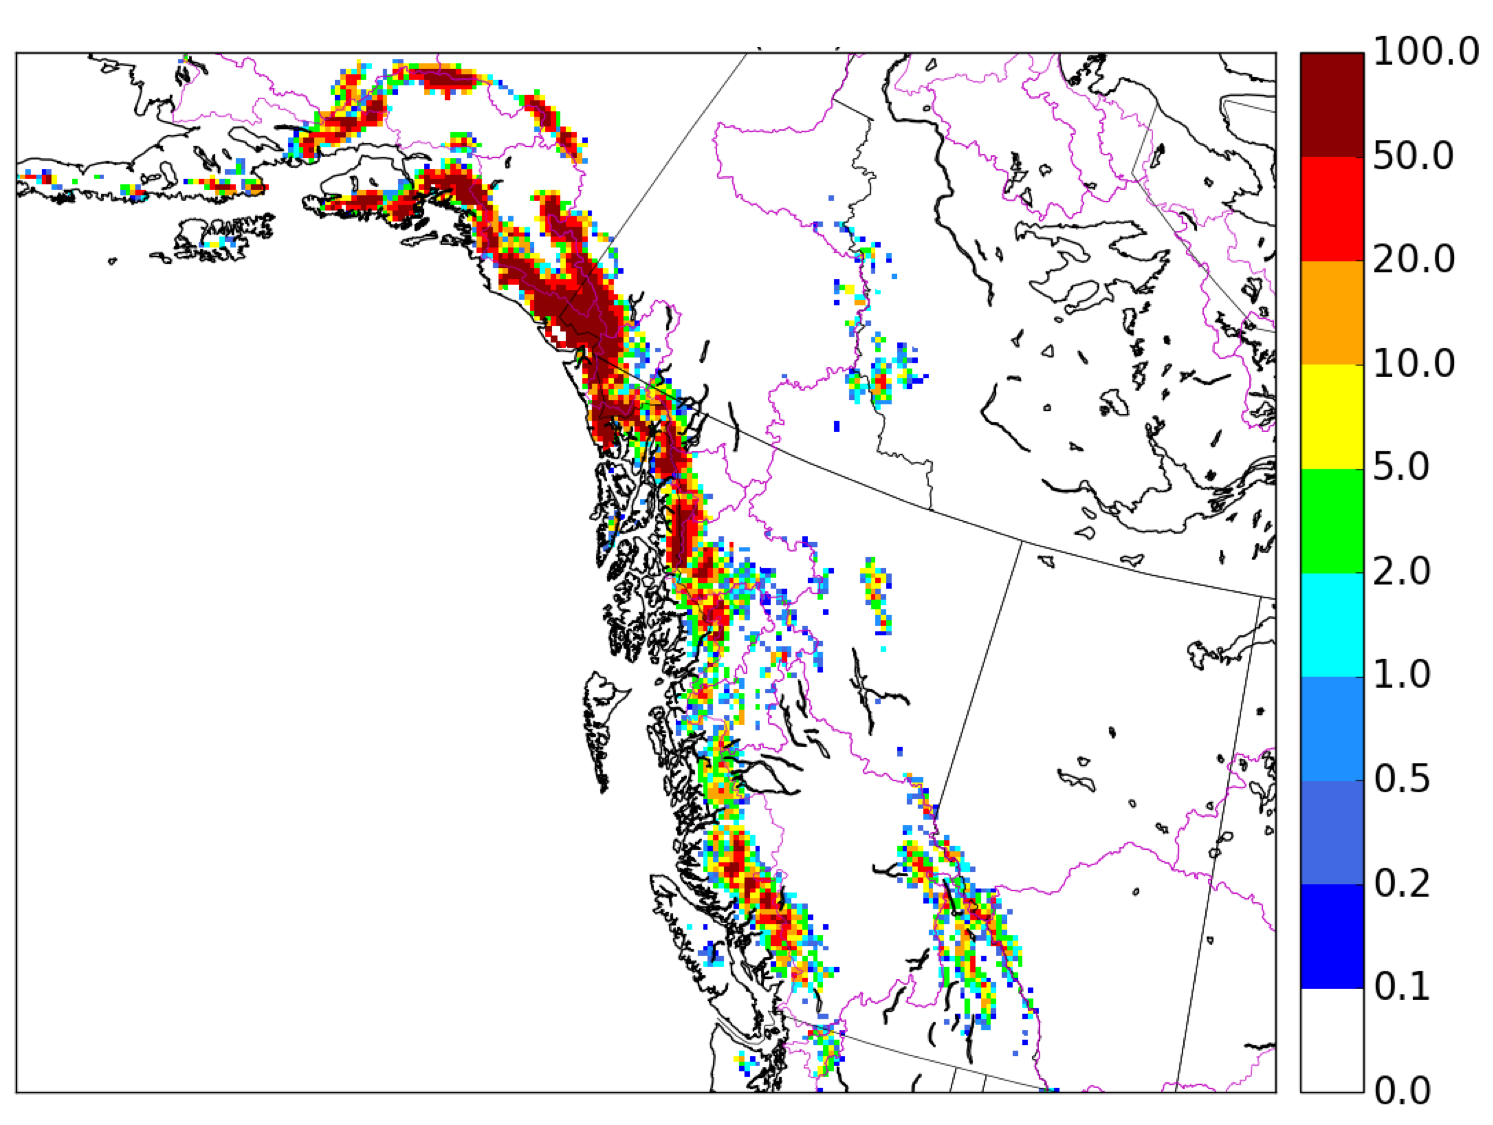
\includegraphics[width=\linewidth]{figures/glacier_fraction}
  \captionof{figure}{\label{figure:glacier_fraction}\color{Green} Spatial extent of glacier fractions used as initial conditions for
                      the WC\_044\_modified and WC\_011\_modified configurations. Based on Randolph
                      Glacier Innventory (RGI) global dataset.}
}






%----------------------------------------------------------------------------------------
%	RESULTS
%----------------------------------------------------------------------------------------

\section*{(C) Results}
\subsection*{C.1 Impact of added parameterizations on seasonal mean fields}
\noindent
\begin{minipage}[t]{\linewidth}
\begin{tikzpicture}
    % schematics
    \node (wc044default) {
      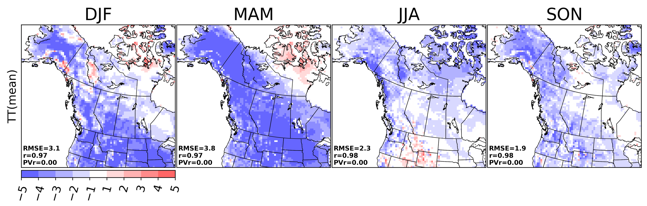
\includegraphics[width=0.95\linewidth, trim={0.3cm 0.1cm 0 0.1cm}, clip]{figures/seasonal_mean_TT_bias_wc_044_default}
    };
    \node[left=0.8cm of wc044default, rotate=90, anchor=north, scale=0.8] (wc044default_label) {WC\_044\_default};

    \node [below=-1.85cm of wc044default, anchor=north] (wc044modified) {
      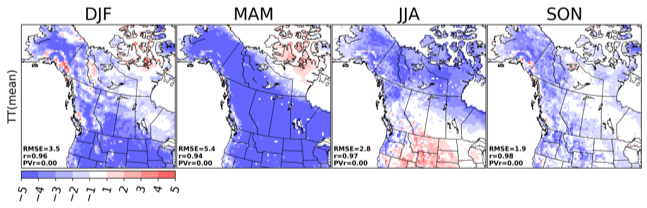
\includegraphics[width=0.95\linewidth, trim={0.3cm 0.1cm 0 0.4cm}, clip]{figures/seasonal_mean_TT_bias_wc_044_modified}
    };
    \node[left=0.8cm of wc044modified, anchor=north, rotate=90, scale=0.8] (wc044modified_label) {WC\_044\_modified};
\end{tikzpicture}
\captionof{figure}{\label{figure:t2mvalidation}
                   \color{Green} Seasonal 2m air temperature biases with respect to aggregated
                    DAYMET dataset ($^\circ$C) for WC\_044\_default (first row) and
                    WC\_044\_modified (second row).}
\end{minipage}

\vspace{1cm}

\noindent
\begin{minipage}[t]{\linewidth}
\begin{tikzpicture}
    \node (wc044default) {
      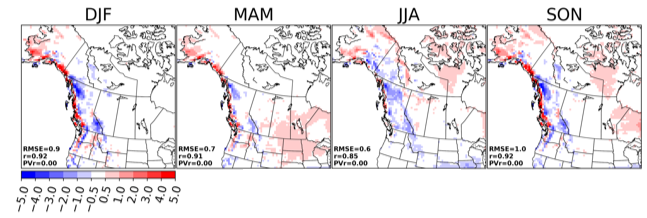
\includegraphics[width=0.95\linewidth, trim={0.35cm 0.3cm 0 0.1cm}, clip]{figures/seasonal_mean_PR_bias_wc_044_default}
    };
    \node[left=0.8cm of wc044default, rotate=90, anchor=north, scale=0.8] (wc044default_label) {WC\_044\_default};

    \node [below=-1.8cm of wc044default, anchor=north] (wc044modified) {
      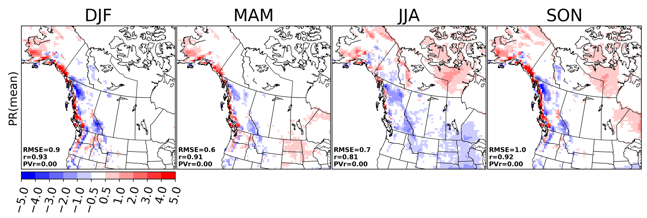
\includegraphics[width=0.95\linewidth, trim={0.35cm 0.1cm 0 0.43cm}, clip]{figures/seasonal_mean_PR_bias_wc_044_modified}
    };
    \node[left=0.8cm of wc044modified, anchor=north, rotate=90, scale=0.8] (wc044modified_label) {WC\_044\_modified};
\end{tikzpicture}
\captionof{figure}{\label{figure:prvalidation}\color{Green} Same as
                   Figure~\ref{figure:t2mvalidation} but for total precipitation (mm/day).}

\end{minipage}


%Discussion
\begin{itemize}
  \item DJF and SON 2m-air temperature and total precipitation are not significantly
  affected by the new parameterizations (See Figures \ref{figure:t2mvalidation} and \ref{figure:prvalidation}).
  \item Although MAM season air temperature cold bias is larger in WC\_044\_modified with respect to WC\_044\_default,
  significant decreases of wet biases in MAM total precipitation in the southwestern part of the domain are noted for  WC\_044\_modified.
  The cold bias in the MAM temperatures is caused by the slow growth rate in the vegetation scheme, which leads to higher albedos and cooler temperatures during MAM.
  \item The new parameterizations produce warmer 2m-air temperatures in the southern part
  of the domain leading to larger positive biases in the southwestern and removing negative biases in
  southeastern parts of the domain.
  \item JJA precipitation is slightly worse in WC\_044\_modified with respect to
  the default configuration in the southeastern part of the domain.
\end{itemize}

\subsection*{C.2 Impact of resolution on seasonal mean 2m-air temperature and total precipitation simulated by the improved model}
\noindent
\begin{minipage}[t]{\linewidth}
\begin{tikzpicture}
      \node (wc044default) {
        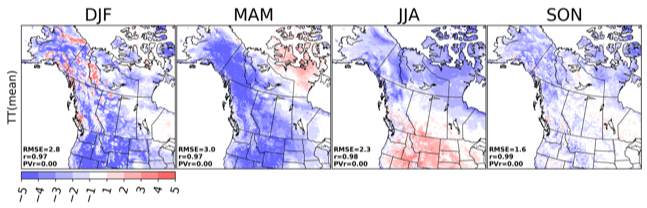
\includegraphics[width=0.95\linewidth, trim={0.3cm 0.1cm 0 0.1cm}, clip]{figures/seasonal_mean_TT_bias_wc_011_modified}
      };
      \node[left=0.8cm of wc044default, rotate=90, anchor=north, scale=0.8] (wc011modified_label) {WC\_011\_modified};
\end{tikzpicture}

\captionof{figure}{\label{figure:t2mvalidation011}\color{Green} Same as the second
                   row in Figure \ref{figure:t2mvalidation} but for WC\_011\_modified ($^\circ$C).}
\end{minipage}


\noindent
\begin{minipage}[t]{\linewidth}
\begin{tikzpicture}
      \node (wc044default) {
        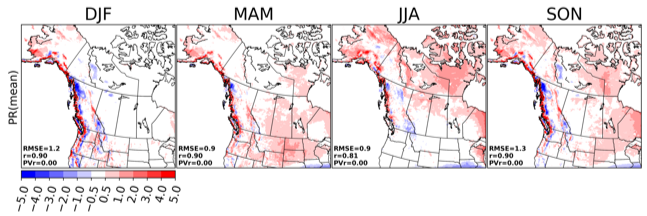
\includegraphics[width=0.95\linewidth, trim={0.33cm 0.1cm 0 0.1cm}, clip]{figures/seasonal_mean_PR_bias_wc_011_modified}
      };
      \node[left=0.8cm of wc044default, rotate=90, anchor=north, scale=0.8] (wc011modified_label) {WC\_011\_modified};
\end{tikzpicture}

\captionof{figure}{\label{figure:prvalidation011}\color{Green} Same as the second
                   row in Figure \ref{figure:prvalidation} but for WC\_011\_modified (mm/day).}
\end{minipage}



\subsection*{C.3 Impact of added parameterizations and of resolution on simulated daily extremes}

To evaluate the impacts of the model modifications on simulated daily extremes the 90th percentile of
daily minimum temperature (TN90), 10th percentile of daily maximum temperature (TX10) and 90th percentile of
daily mean total precipitation (PR90) are averaged over land and the time series are compared for WC\_044\_default and
WC\_044\_modified. The indices are calculated as in \citet{curry2016}.

\noindent
\begin{minipage}[t]{\linewidth}
\center
\begin{tikzpicture}
    % schematics
    \node[label={\small TX10}] (tx10) {
      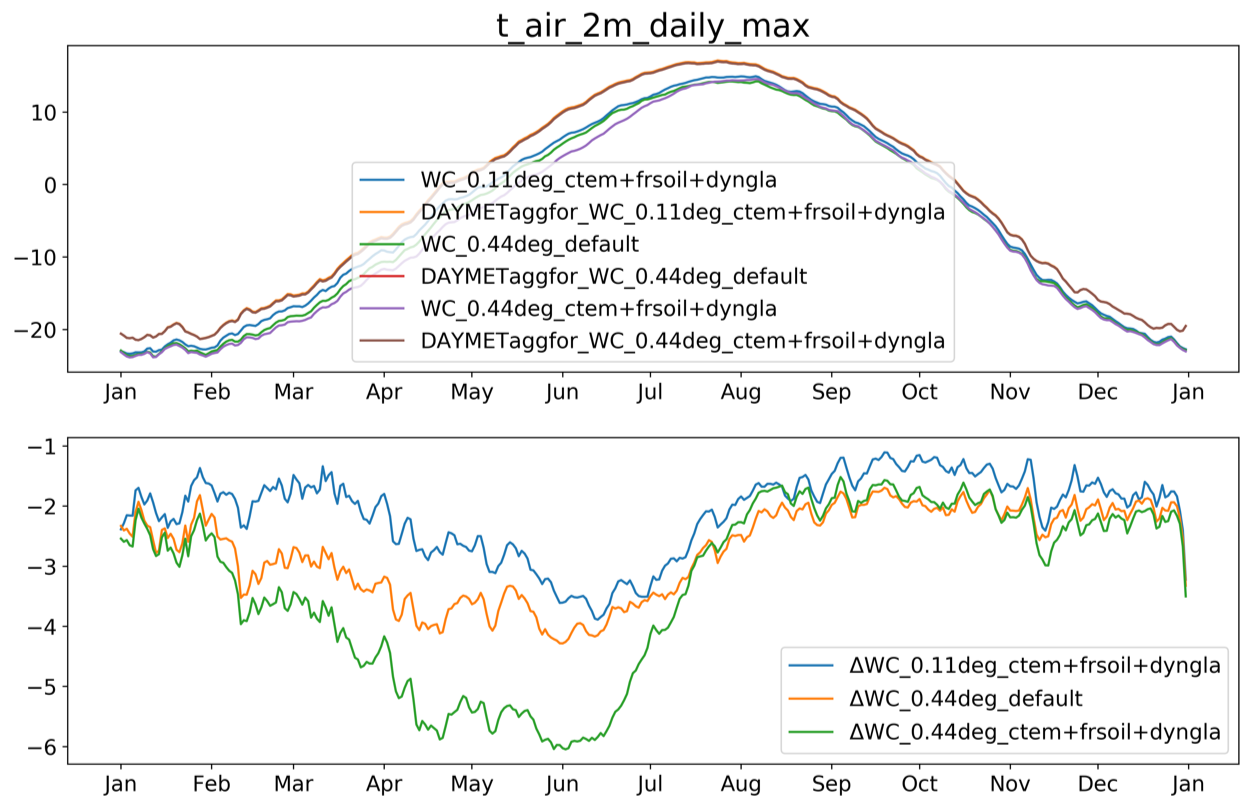
\includegraphics[width=0.48\linewidth, trim={0 0 0 0}, clip]{figures/tx10_ts}
    };
    \node[right=0.1cm of tx10.east, anchor=west, label={\small TN90}] (tn90) {
      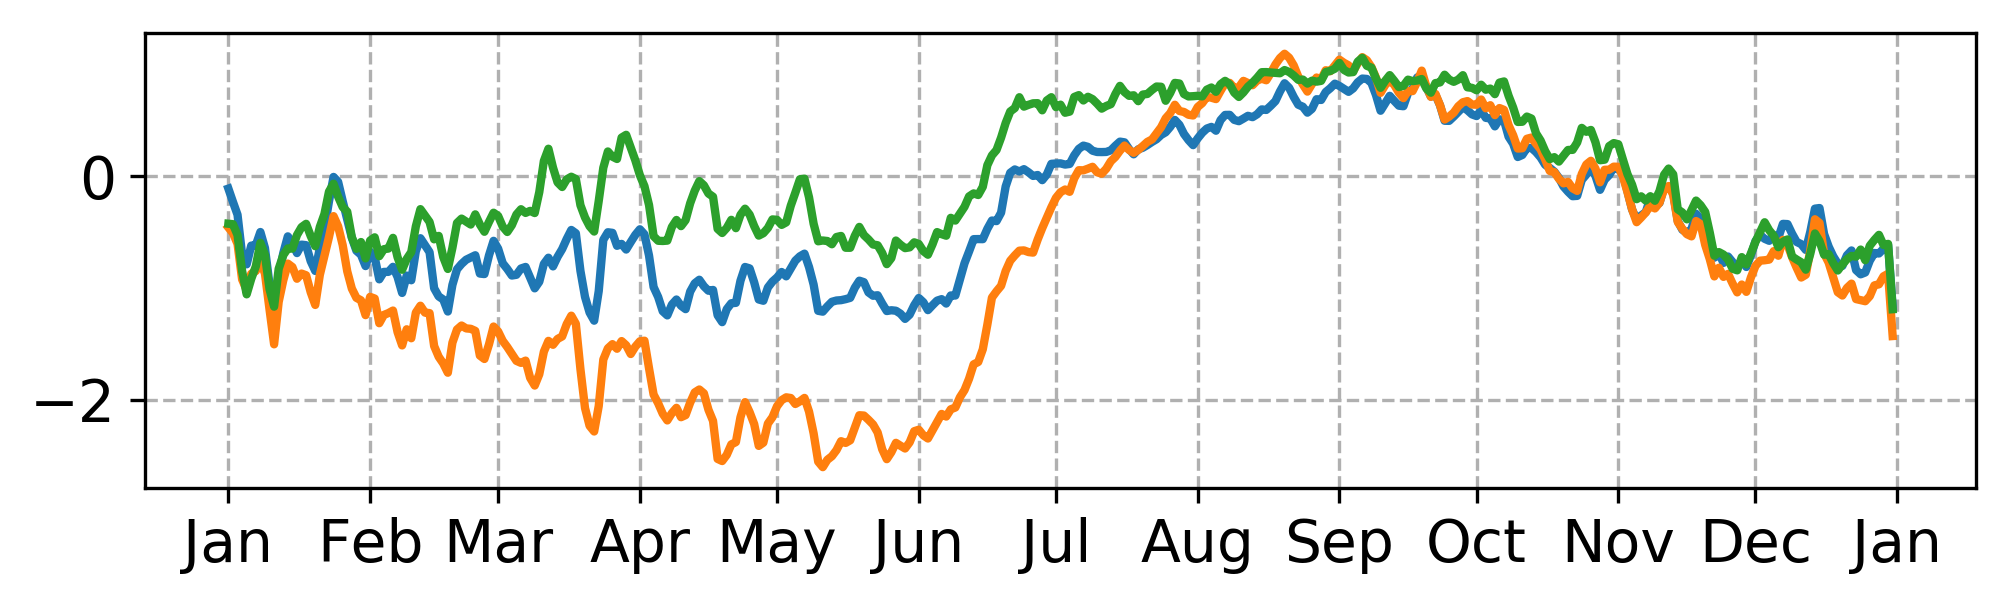
\includegraphics[width=0.48\linewidth, trim={0 0 0 0}, clip]{figures/tn90_ts}
    };

    \node[label={\small PR90}, below=1cm of tx10.south, anchor=north] (pr90) {
      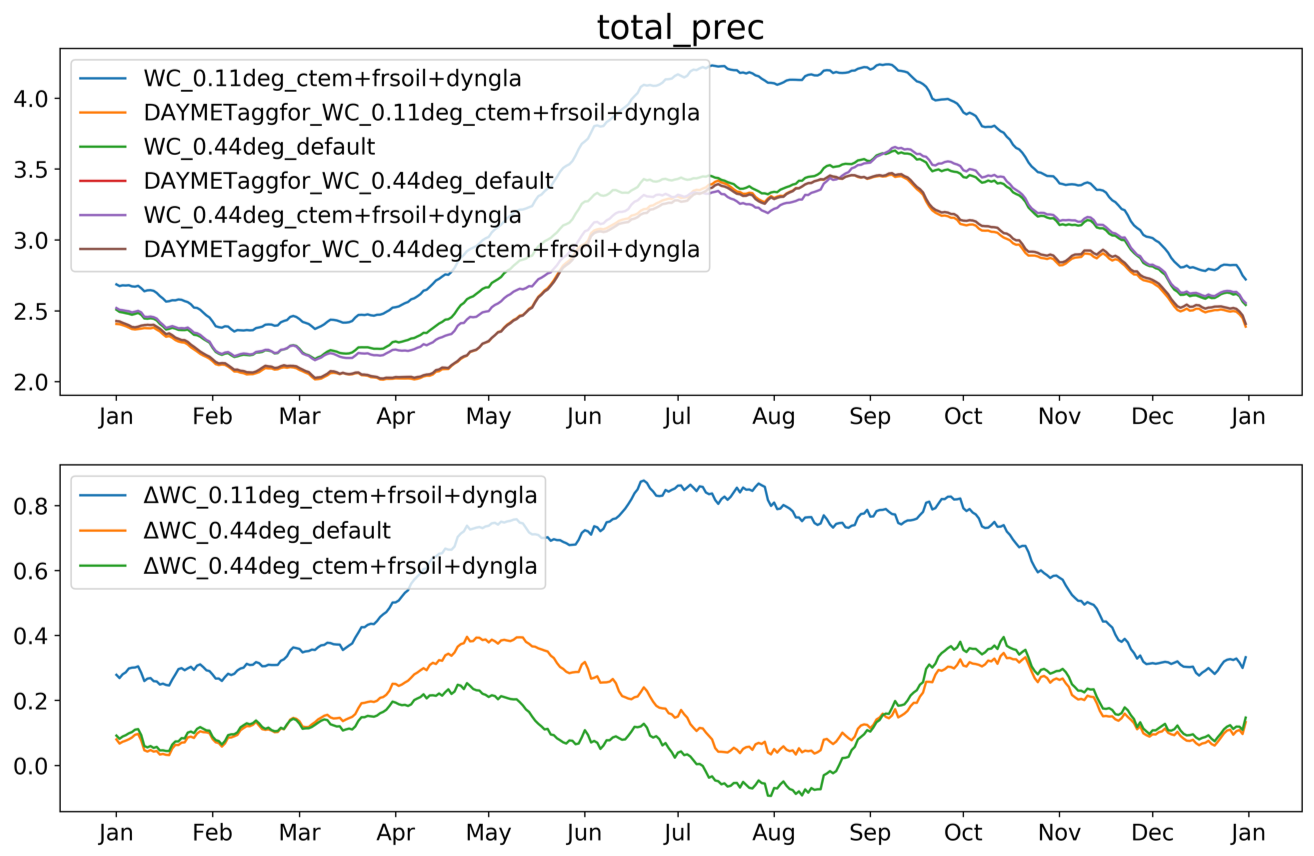
\includegraphics[width=0.48\linewidth, trim={0 0 0 0}, clip]{figures/pr90_ts}
    };

    \node [below=-1cm of tn90.south, anchor=north, text width=0.4\linewidth, align=left]{
      \captionof{figure}{\color{Green} Area averaged biases of 10th percentile of daily maximum temperature (TX10),
      90th percentile of daily minimum temperature (TN90) and 90th percentile of daily mean total precipitation (PR90) for WC\_044\_default (blue),
      WC\_044\_modified (orange) and WC\_011\_modified (green). The biases are calculated using DAYMET observation dataset.
      }
    };
\end{tikzpicture}
\end{minipage}


\begin{itemize}
    \item Discussion

\end{itemize}

\subsection*{C.4 Zonal structure of the daily extremes in a region with complex topography}

\noindent
\adjustbox{valign=t, minipage=0.2\linewidth}{
  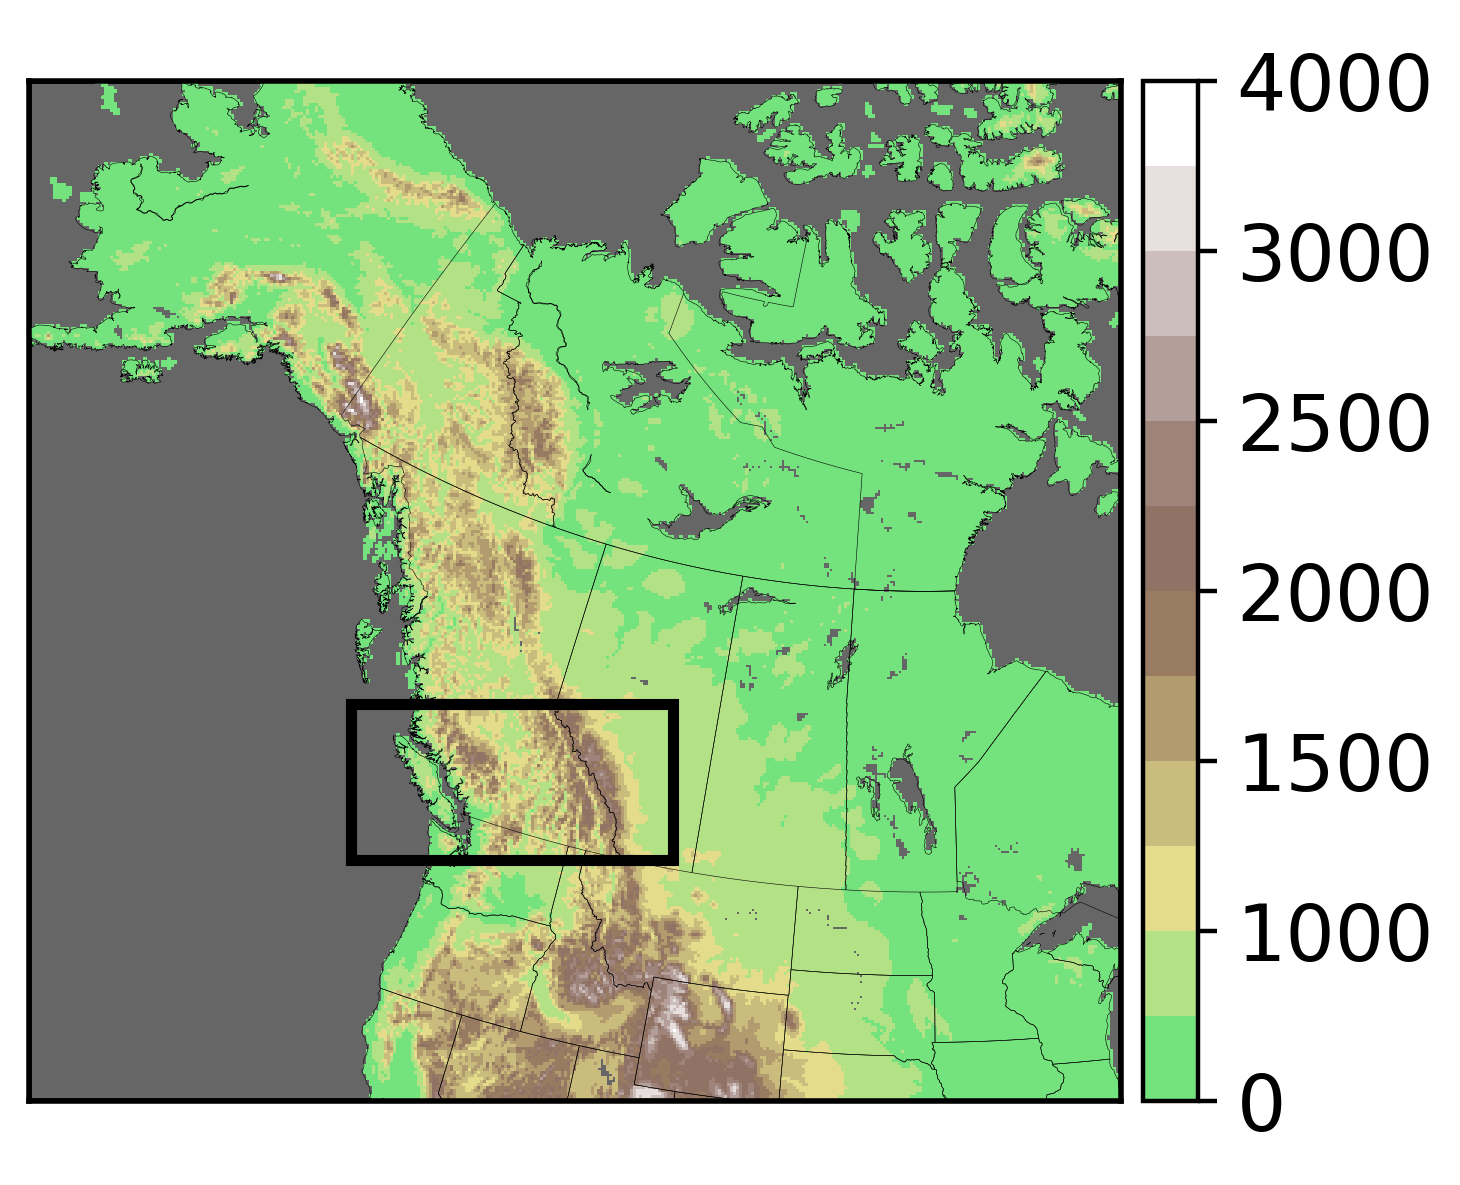
\includegraphics[width=\linewidth, trim={0 0 2.1cm 0}, clip]{figures/domain_and_focus_for_meridional_avg}
}
%
\hfill
%
\adjustbox{valign=t, minipage=0.3\linewidth}{
  \captionof{figure}{\color{Green} Topography field (m) is shown in colors. Black rectangle is showing the region of meridional averaging.}
}
%
\hfill
%
\adjustbox{valign=t, minipage=0.45\linewidth}{
  Discussion
}

\noindent
\begin{minipage}[t]{\linewidth}
\begin{center}

\begin{tikzpicture}
    % TX10
    \node[label={\small TX10 ($^\circ$C)}, label={[rotate=90, anchor=south, yshift=-0.5cm]left:\small DJF}] (tx10_djf) {
      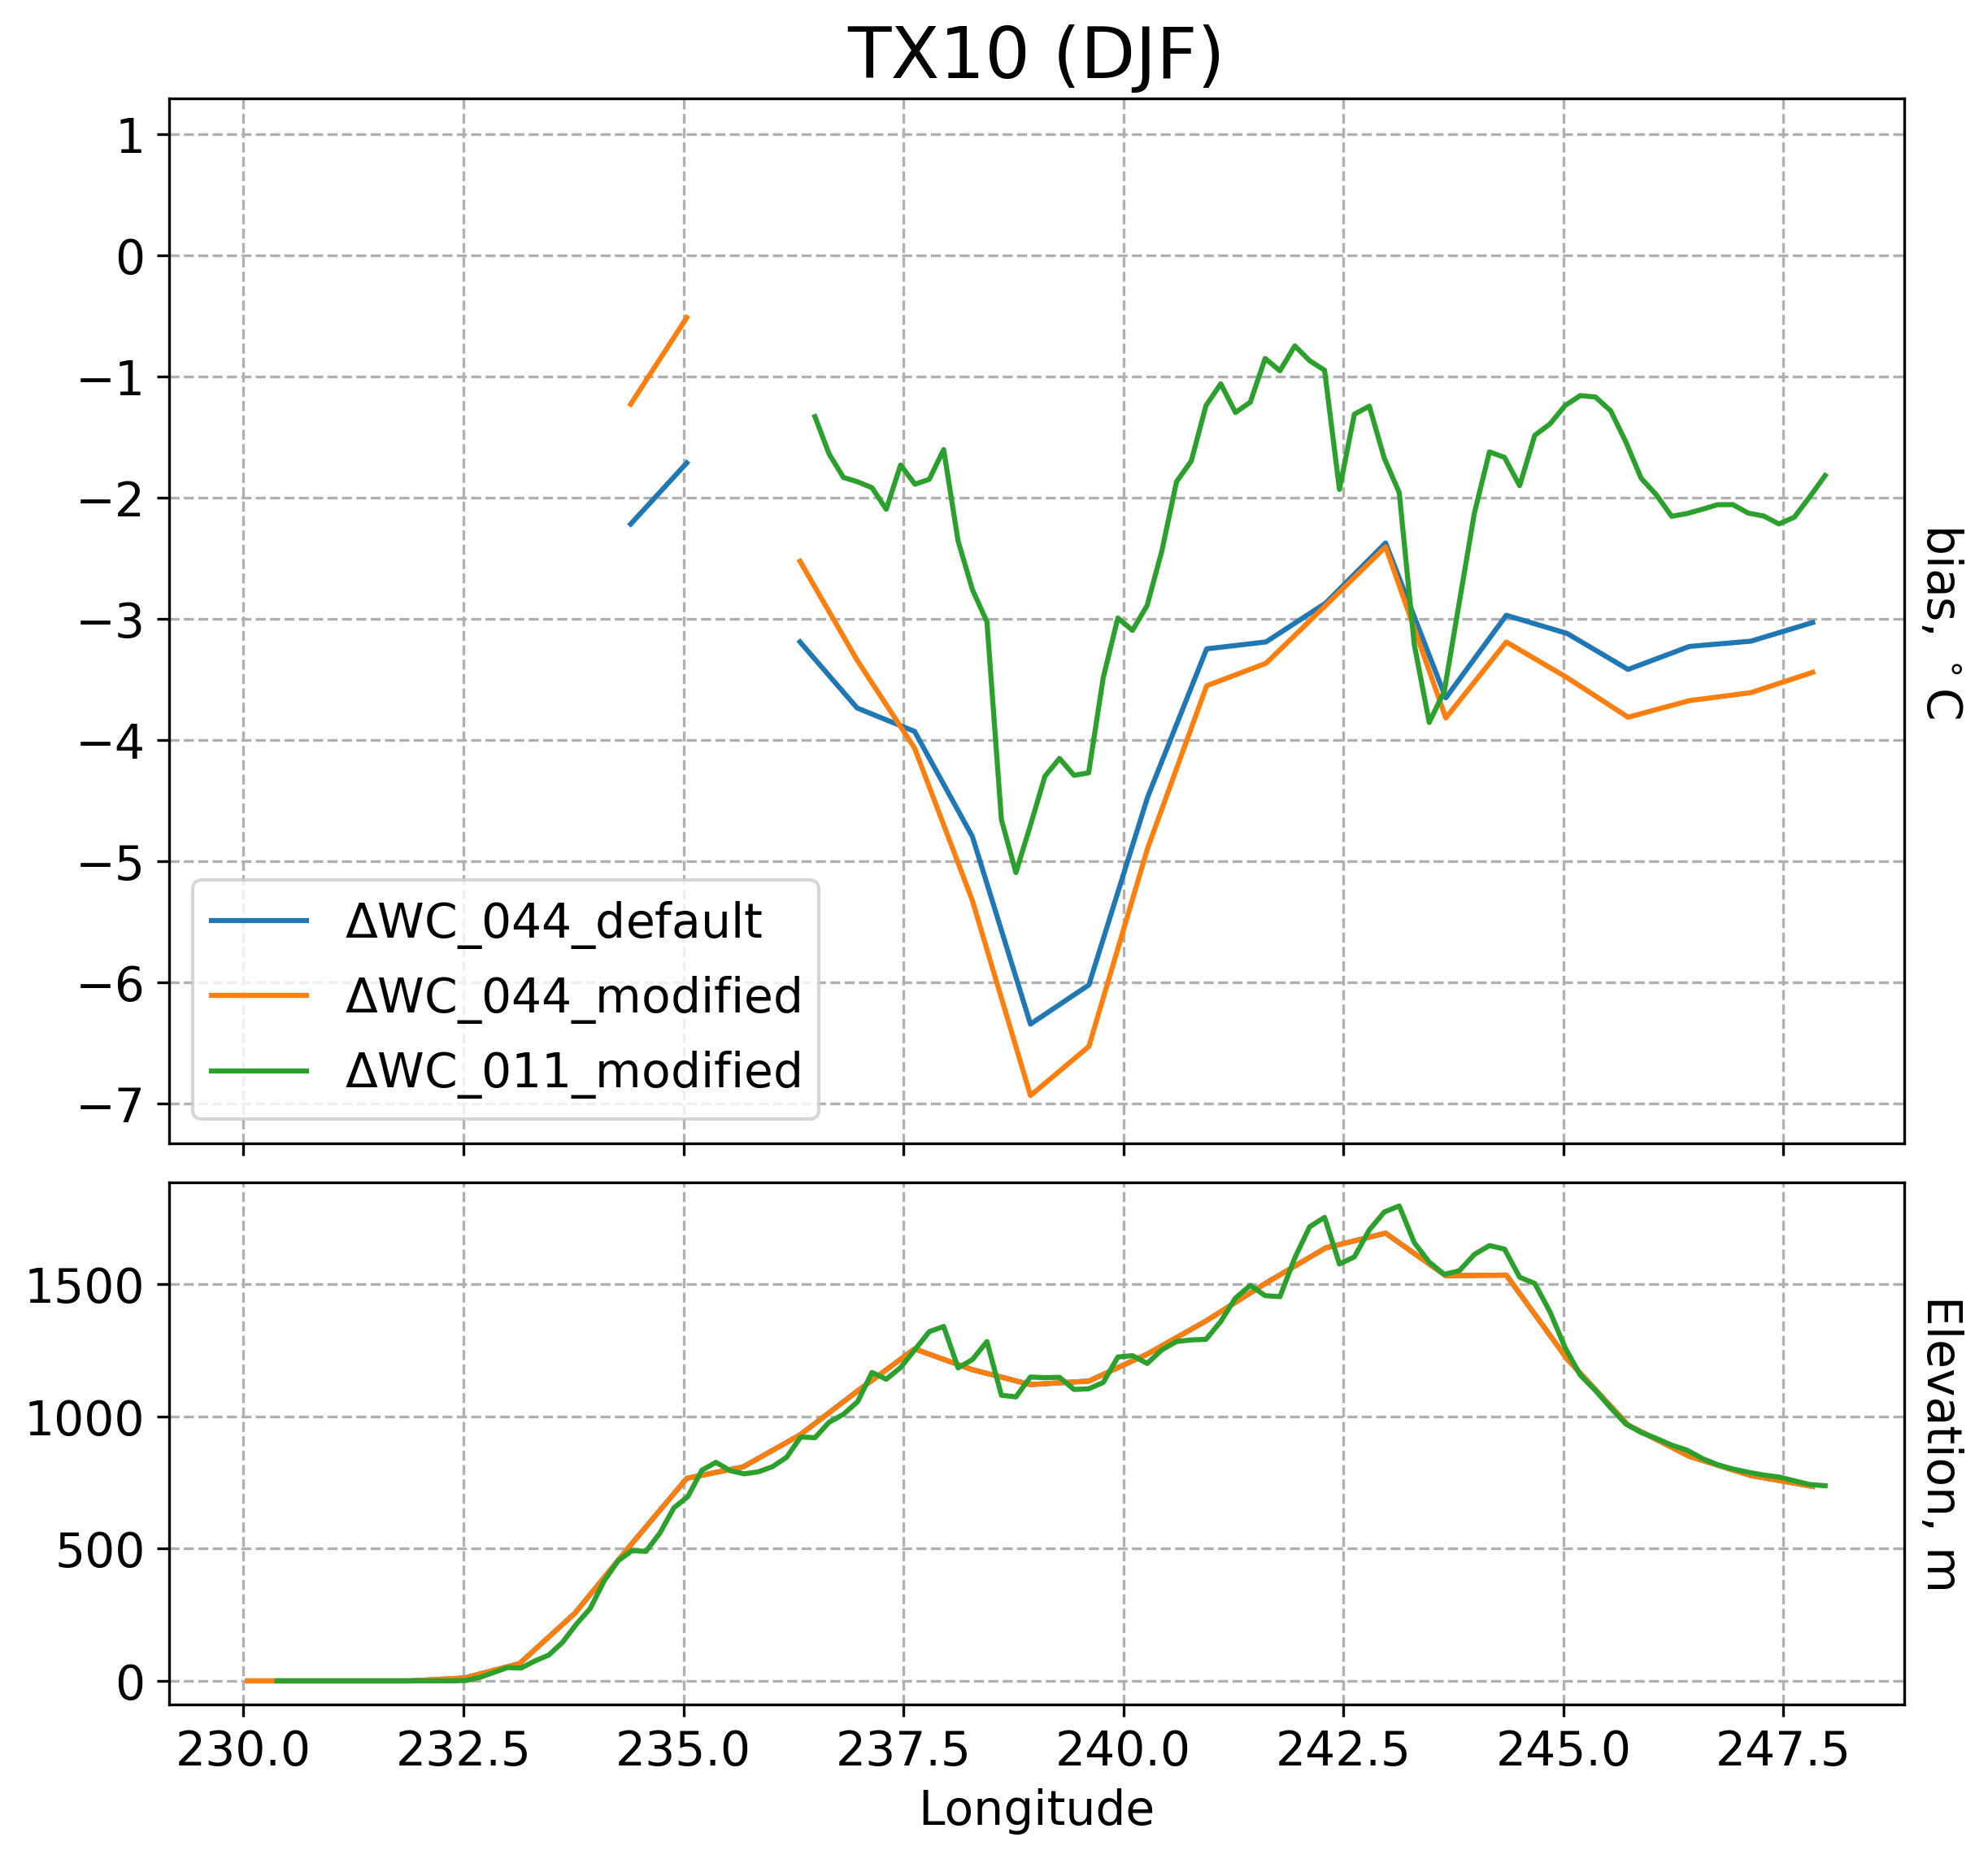
\includegraphics[width=0.31\linewidth, trim={0 8cm 0 0cm}, clip]{figures/meridional_avg/DJF_t_air_2m_daily_max}
    };


    \node[label={[rotate=90, anchor=south, yshift=-0.5cm]left:\small MAM}, below=\hspc of tx10_djf] (tx10_mam) {
      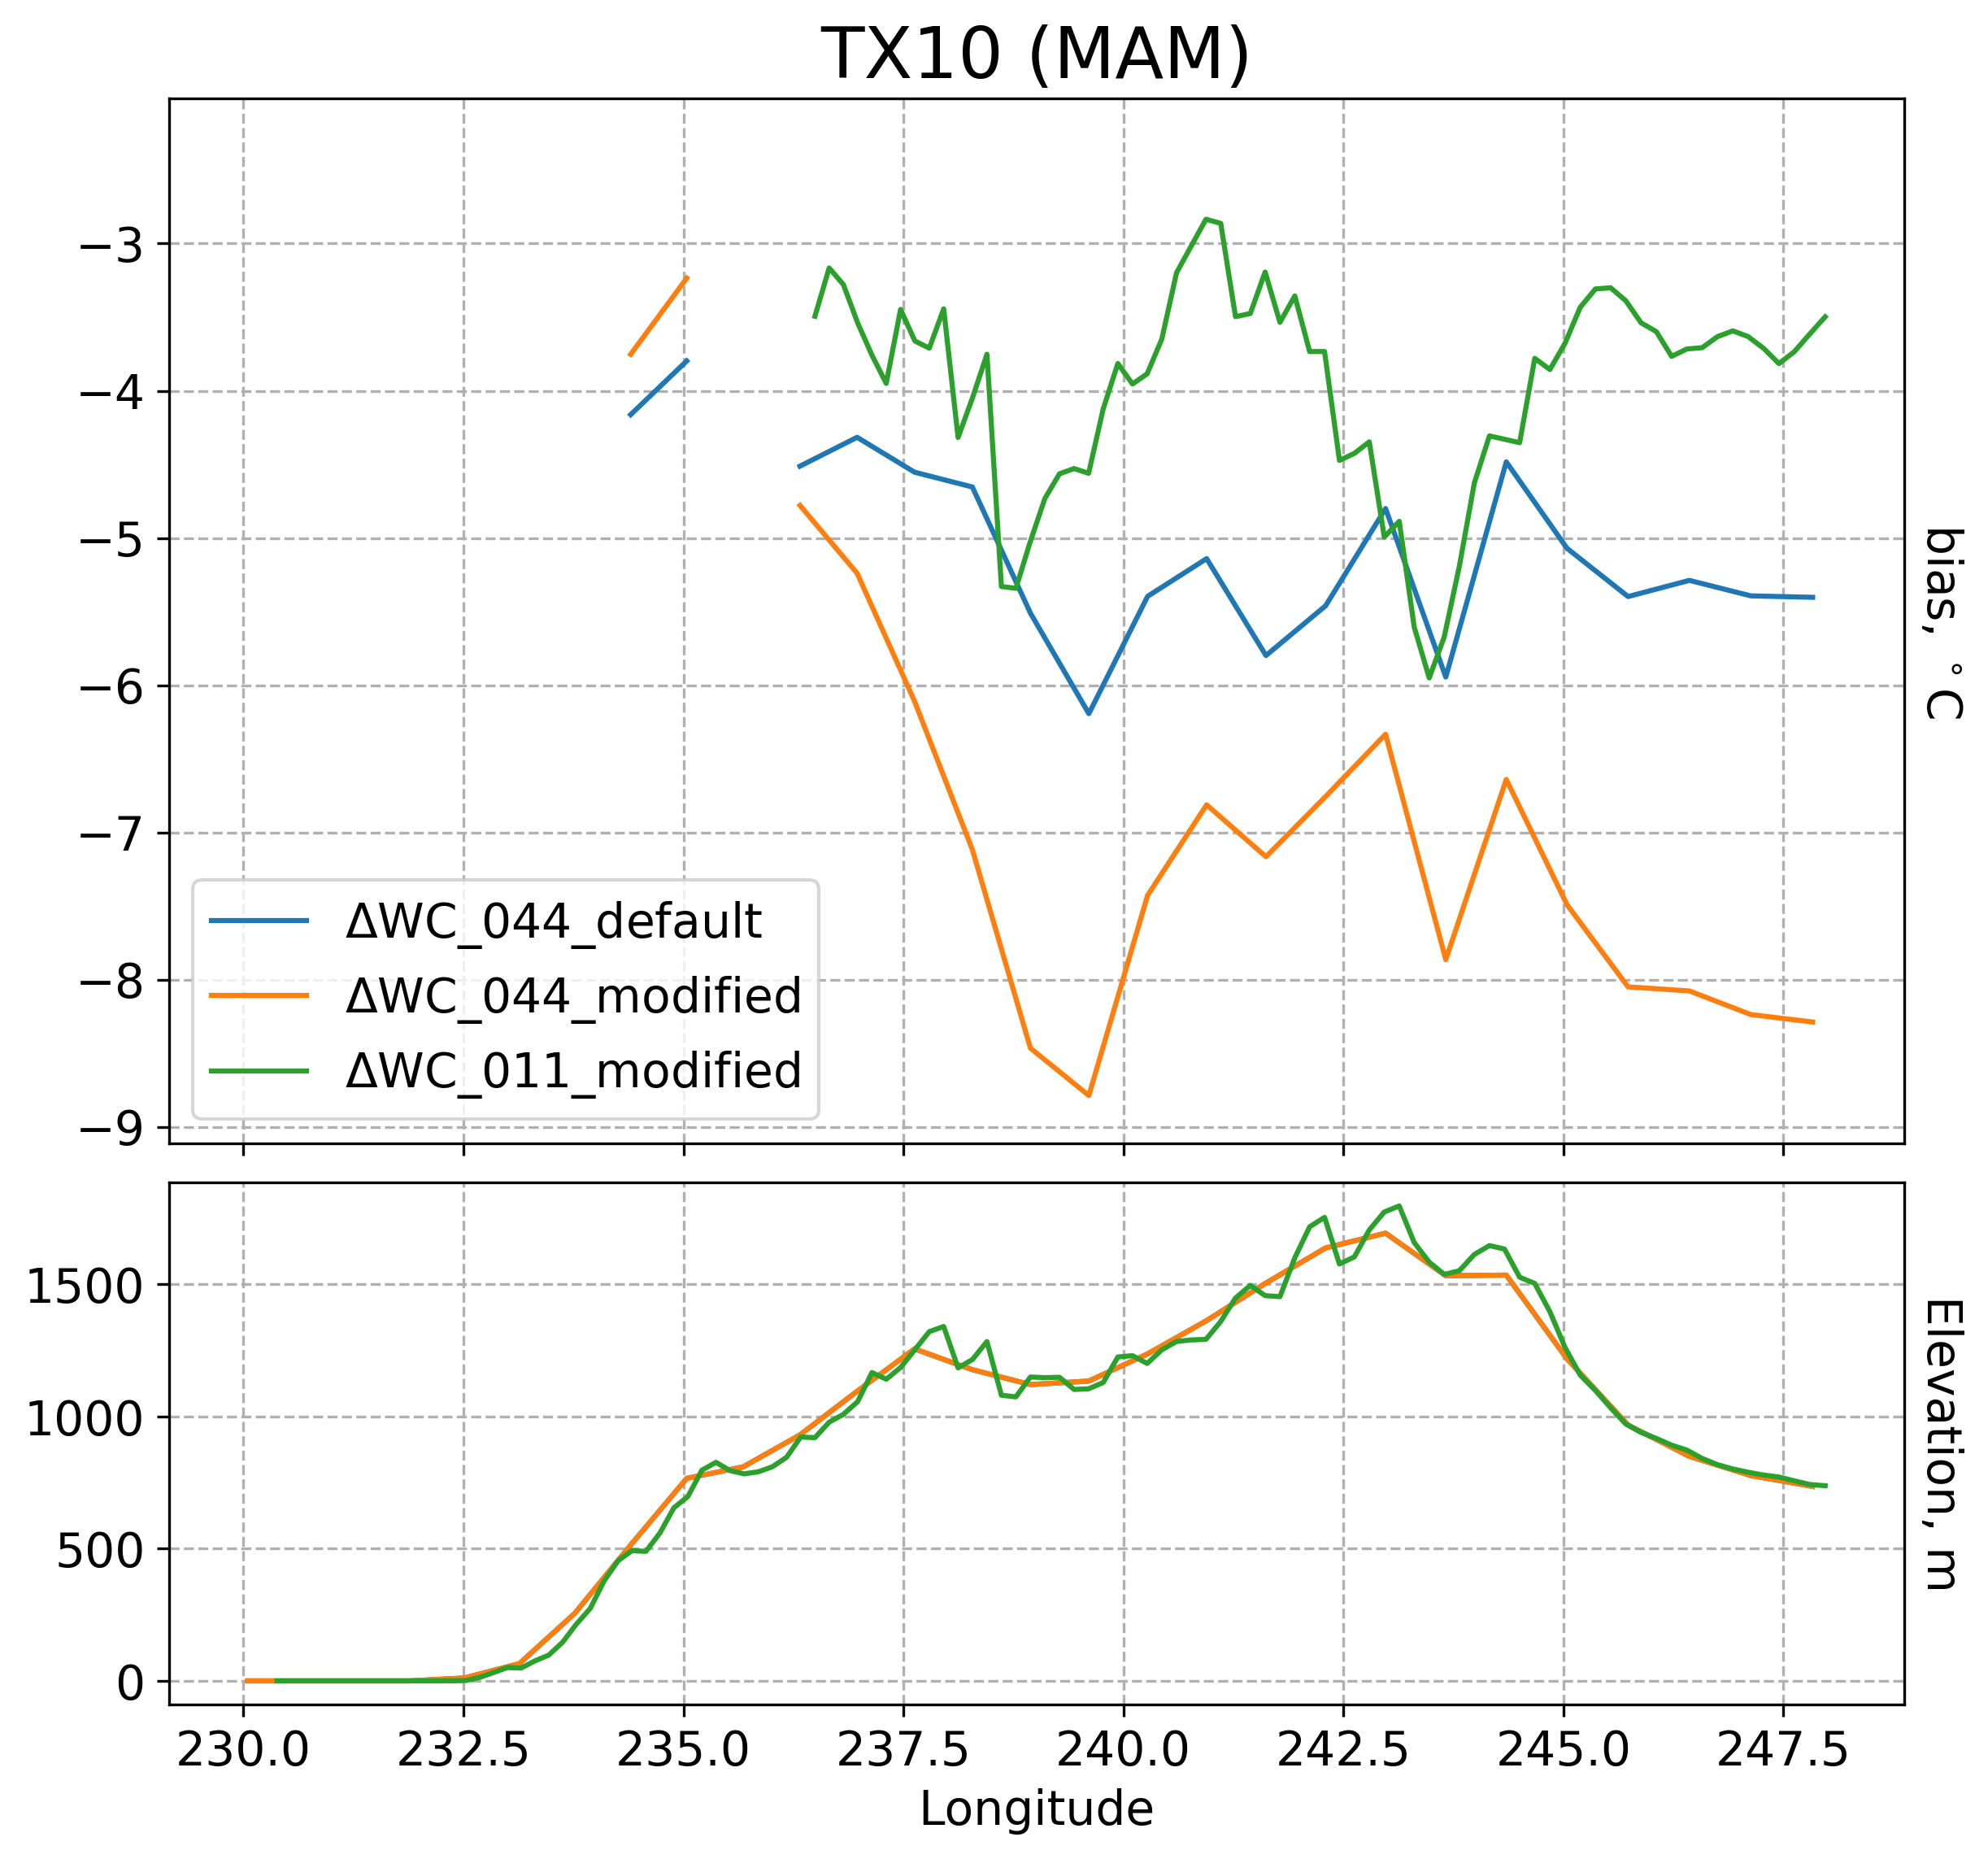
\includegraphics[width=0.31\linewidth, trim={0 8cm 0 0cm}, clip]{figures/meridional_avg/MAM_t_air_2m_daily_max}
    };

    \node[label={[rotate=90, anchor=south, yshift=-0.5cm]left:\small JJA}, below=\hspc of tx10_mam] (tx10_jja) {
      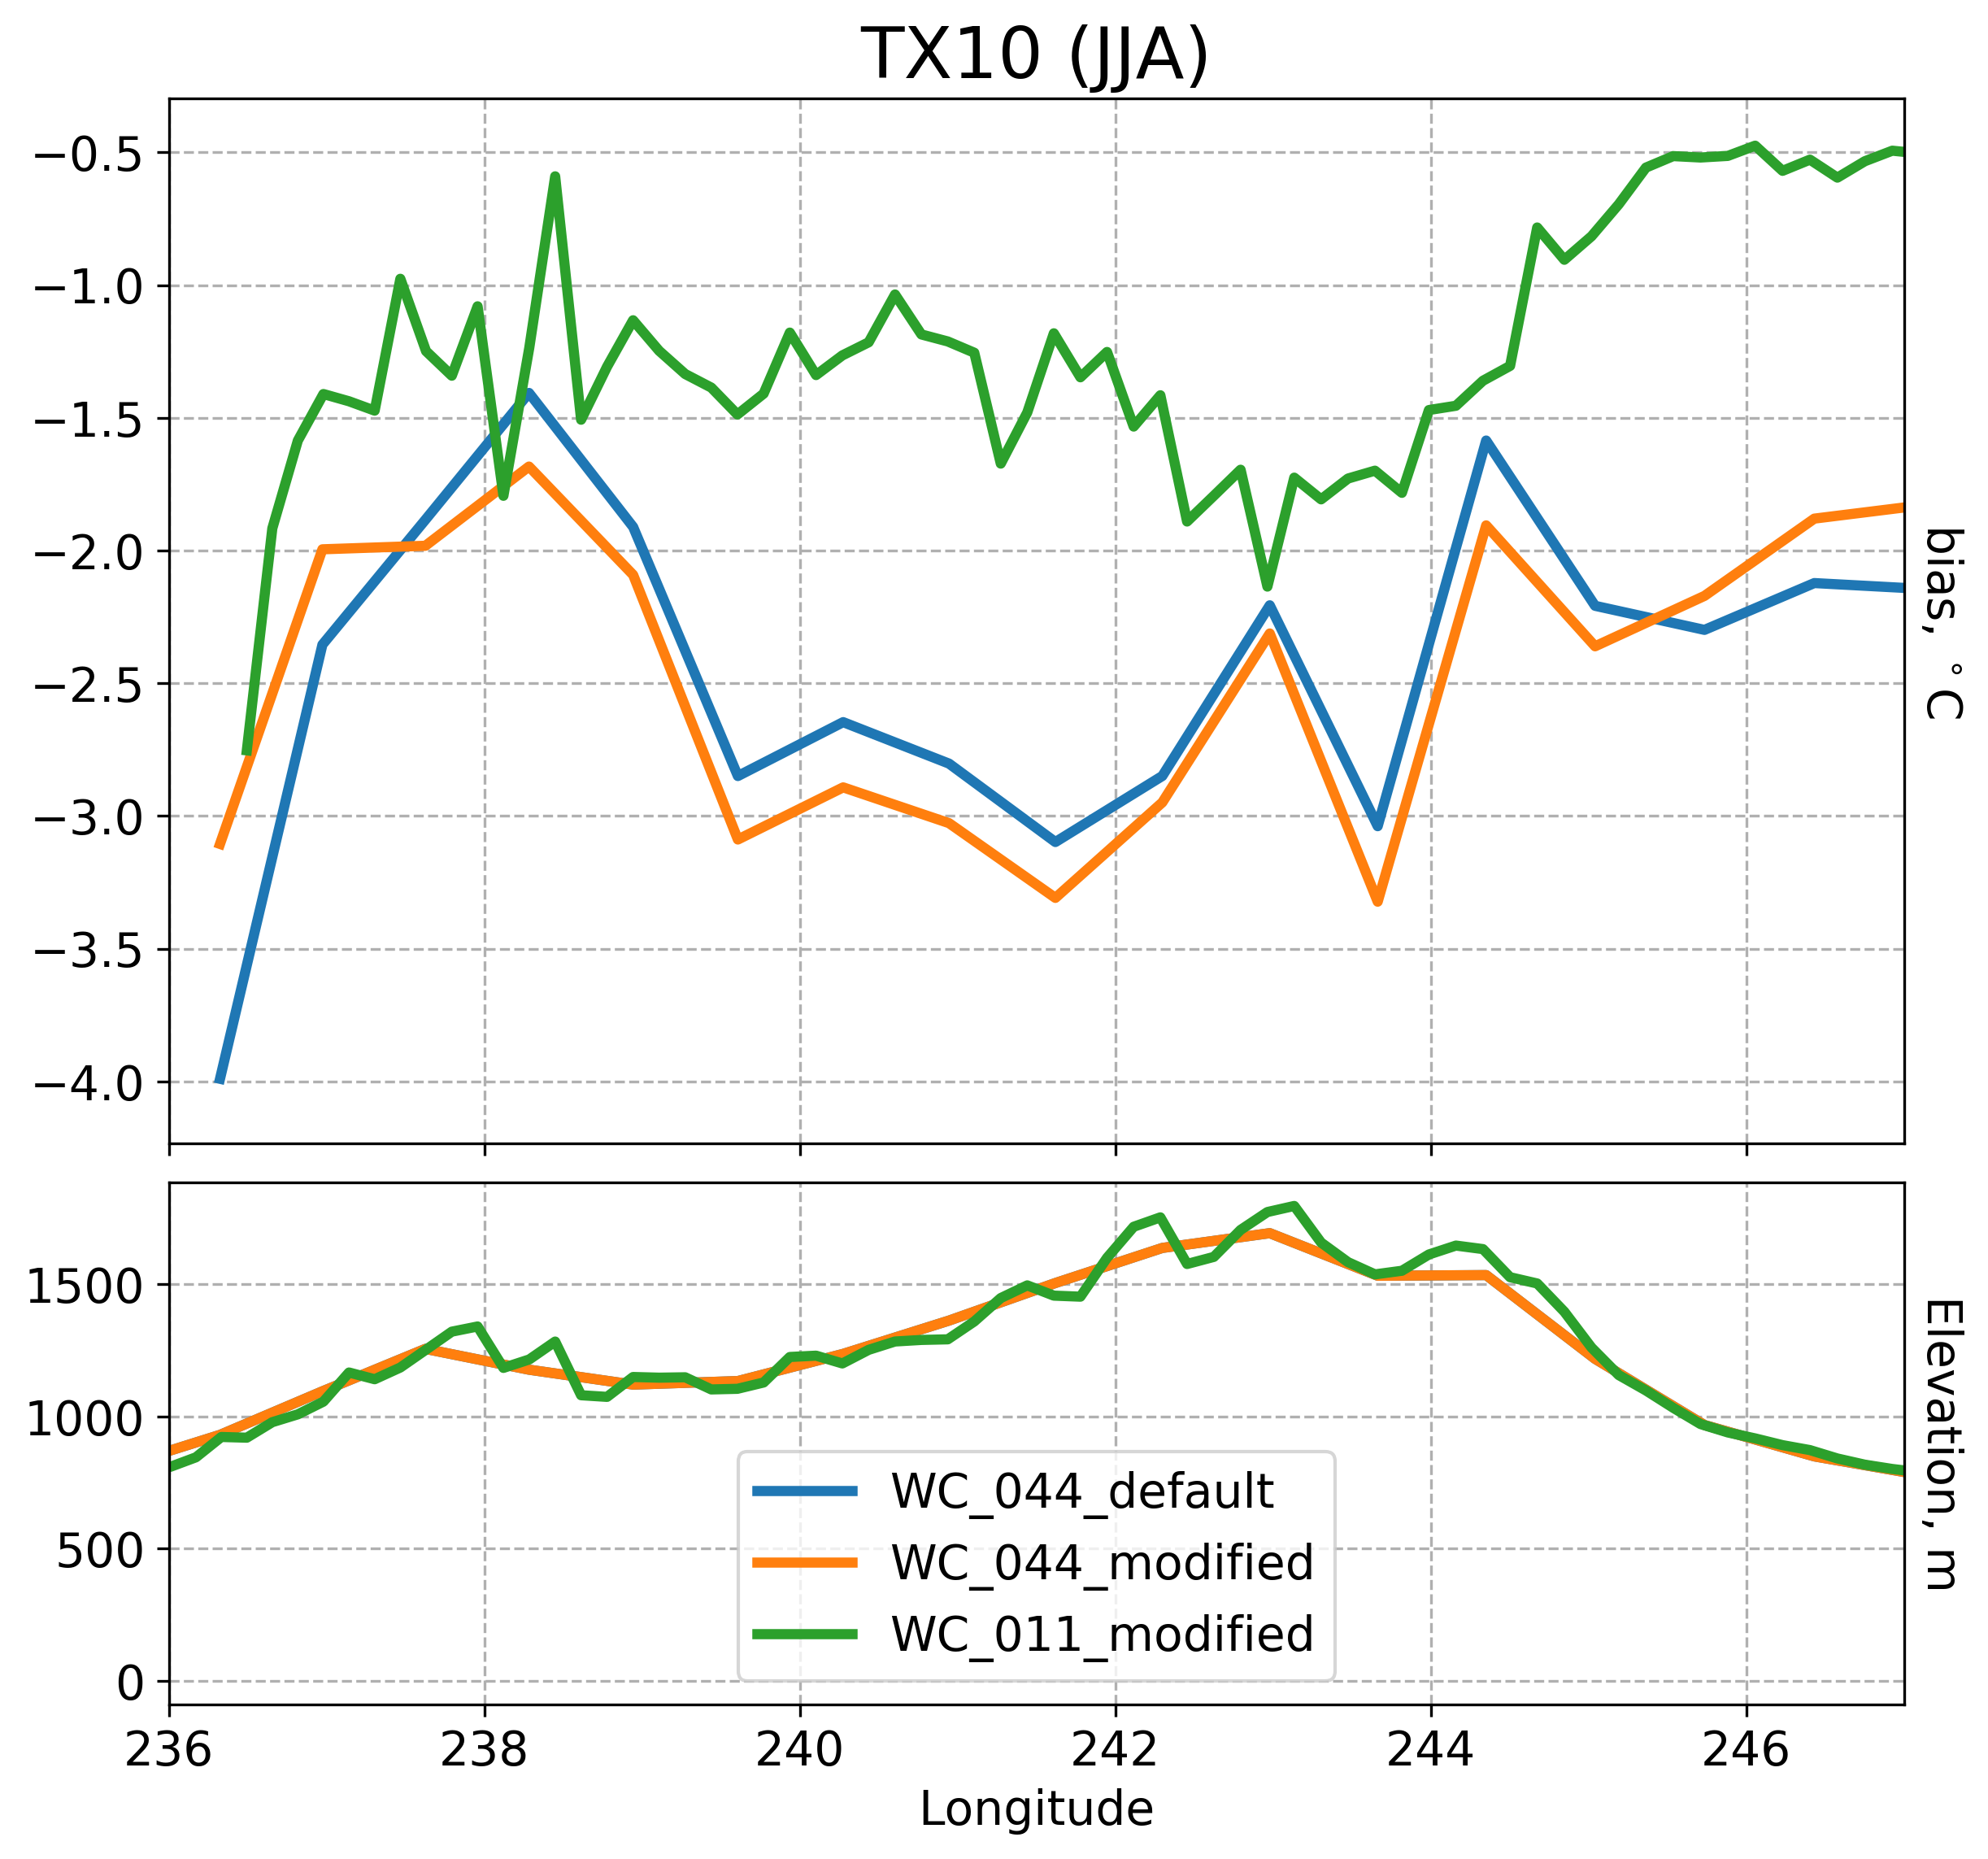
\includegraphics[width=0.31\linewidth, trim={0 8cm 0 0cm}, clip]{figures/meridional_avg/JJA_t_air_2m_daily_max}
    };

    \node[label={[rotate=90, anchor=south, xshift=3cm, yshift=-0.5cm]left:\small SON},below=\hspc of tx10_jja] (tx10_son) {
      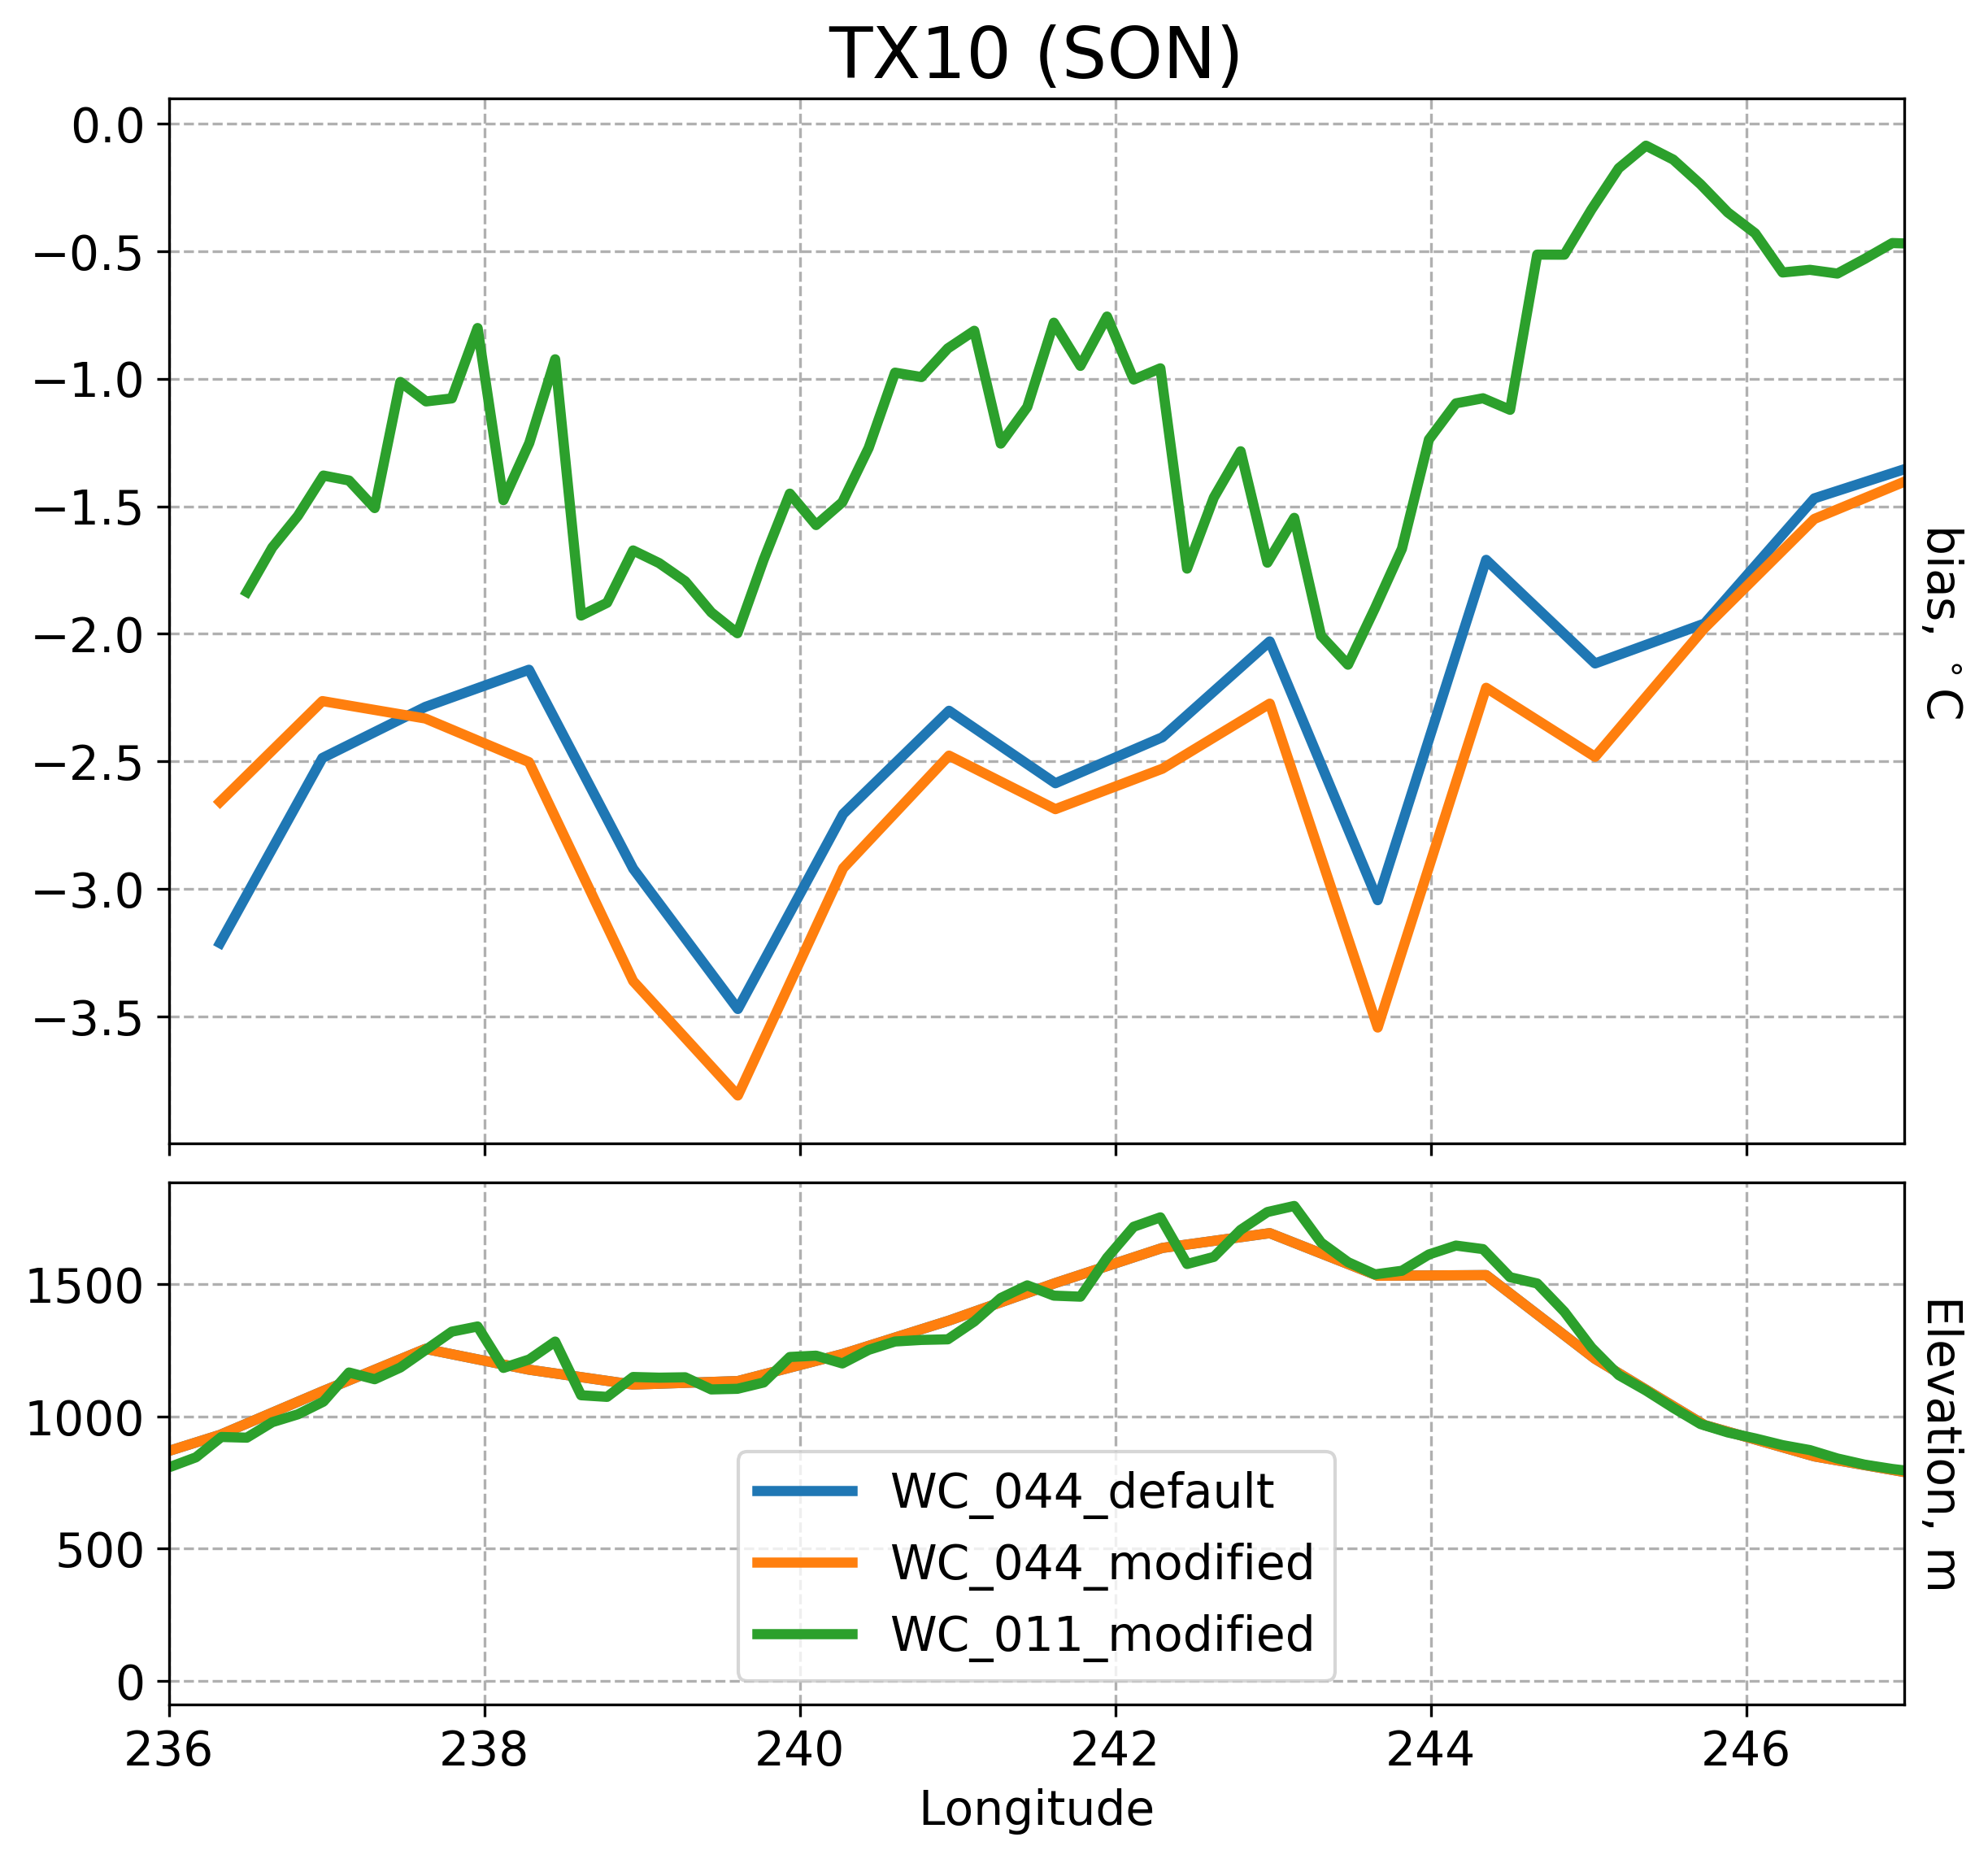
\includegraphics[width=0.31\linewidth, trim={0 0cm 0 0cm}, clip]{figures/meridional_avg/SON_t_air_2m_daily_max}
    };


    %TN90
    \node[label={\small TN90}, right=\wspc of tx10_djf.east, anchor=west] (tn90_djf) {
      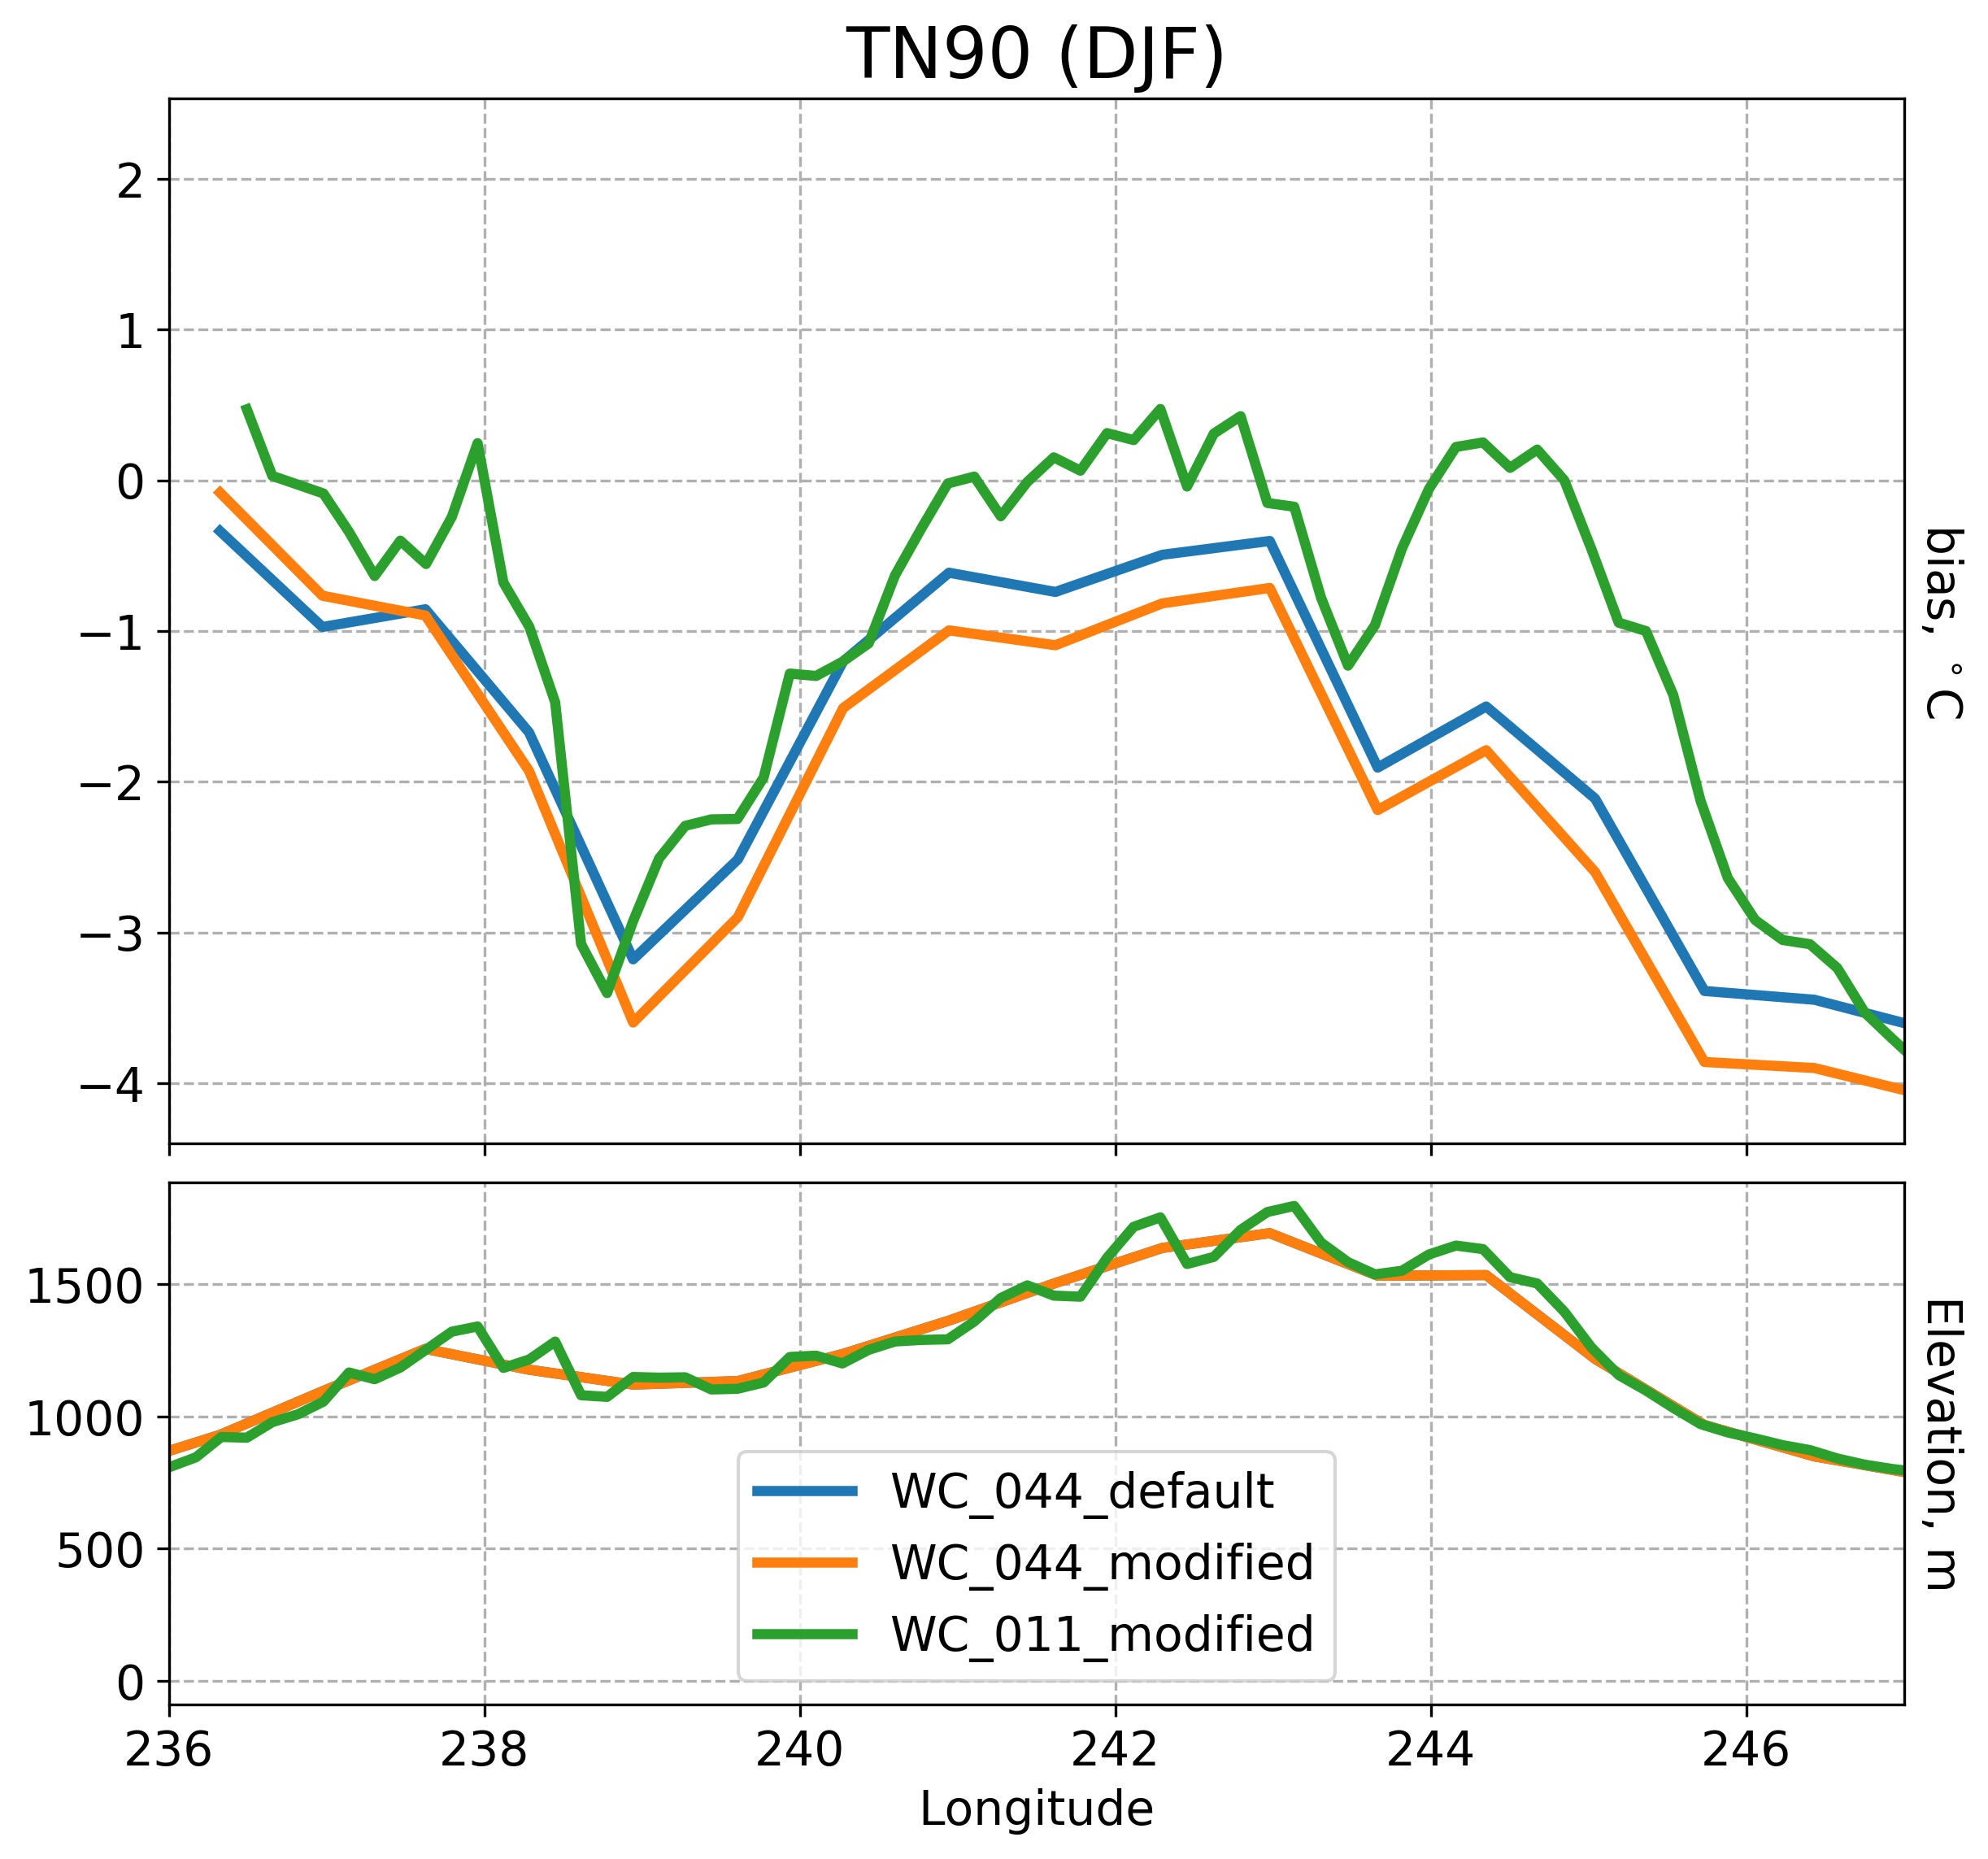
\includegraphics[width=0.31\linewidth, trim={0 8cm 0 0cm}, clip]{figures/meridional_avg/DJF_t_air_2m_daily_min}
    };

    \node[below=\hspc of tn90_djf] (tn90_mam) {
      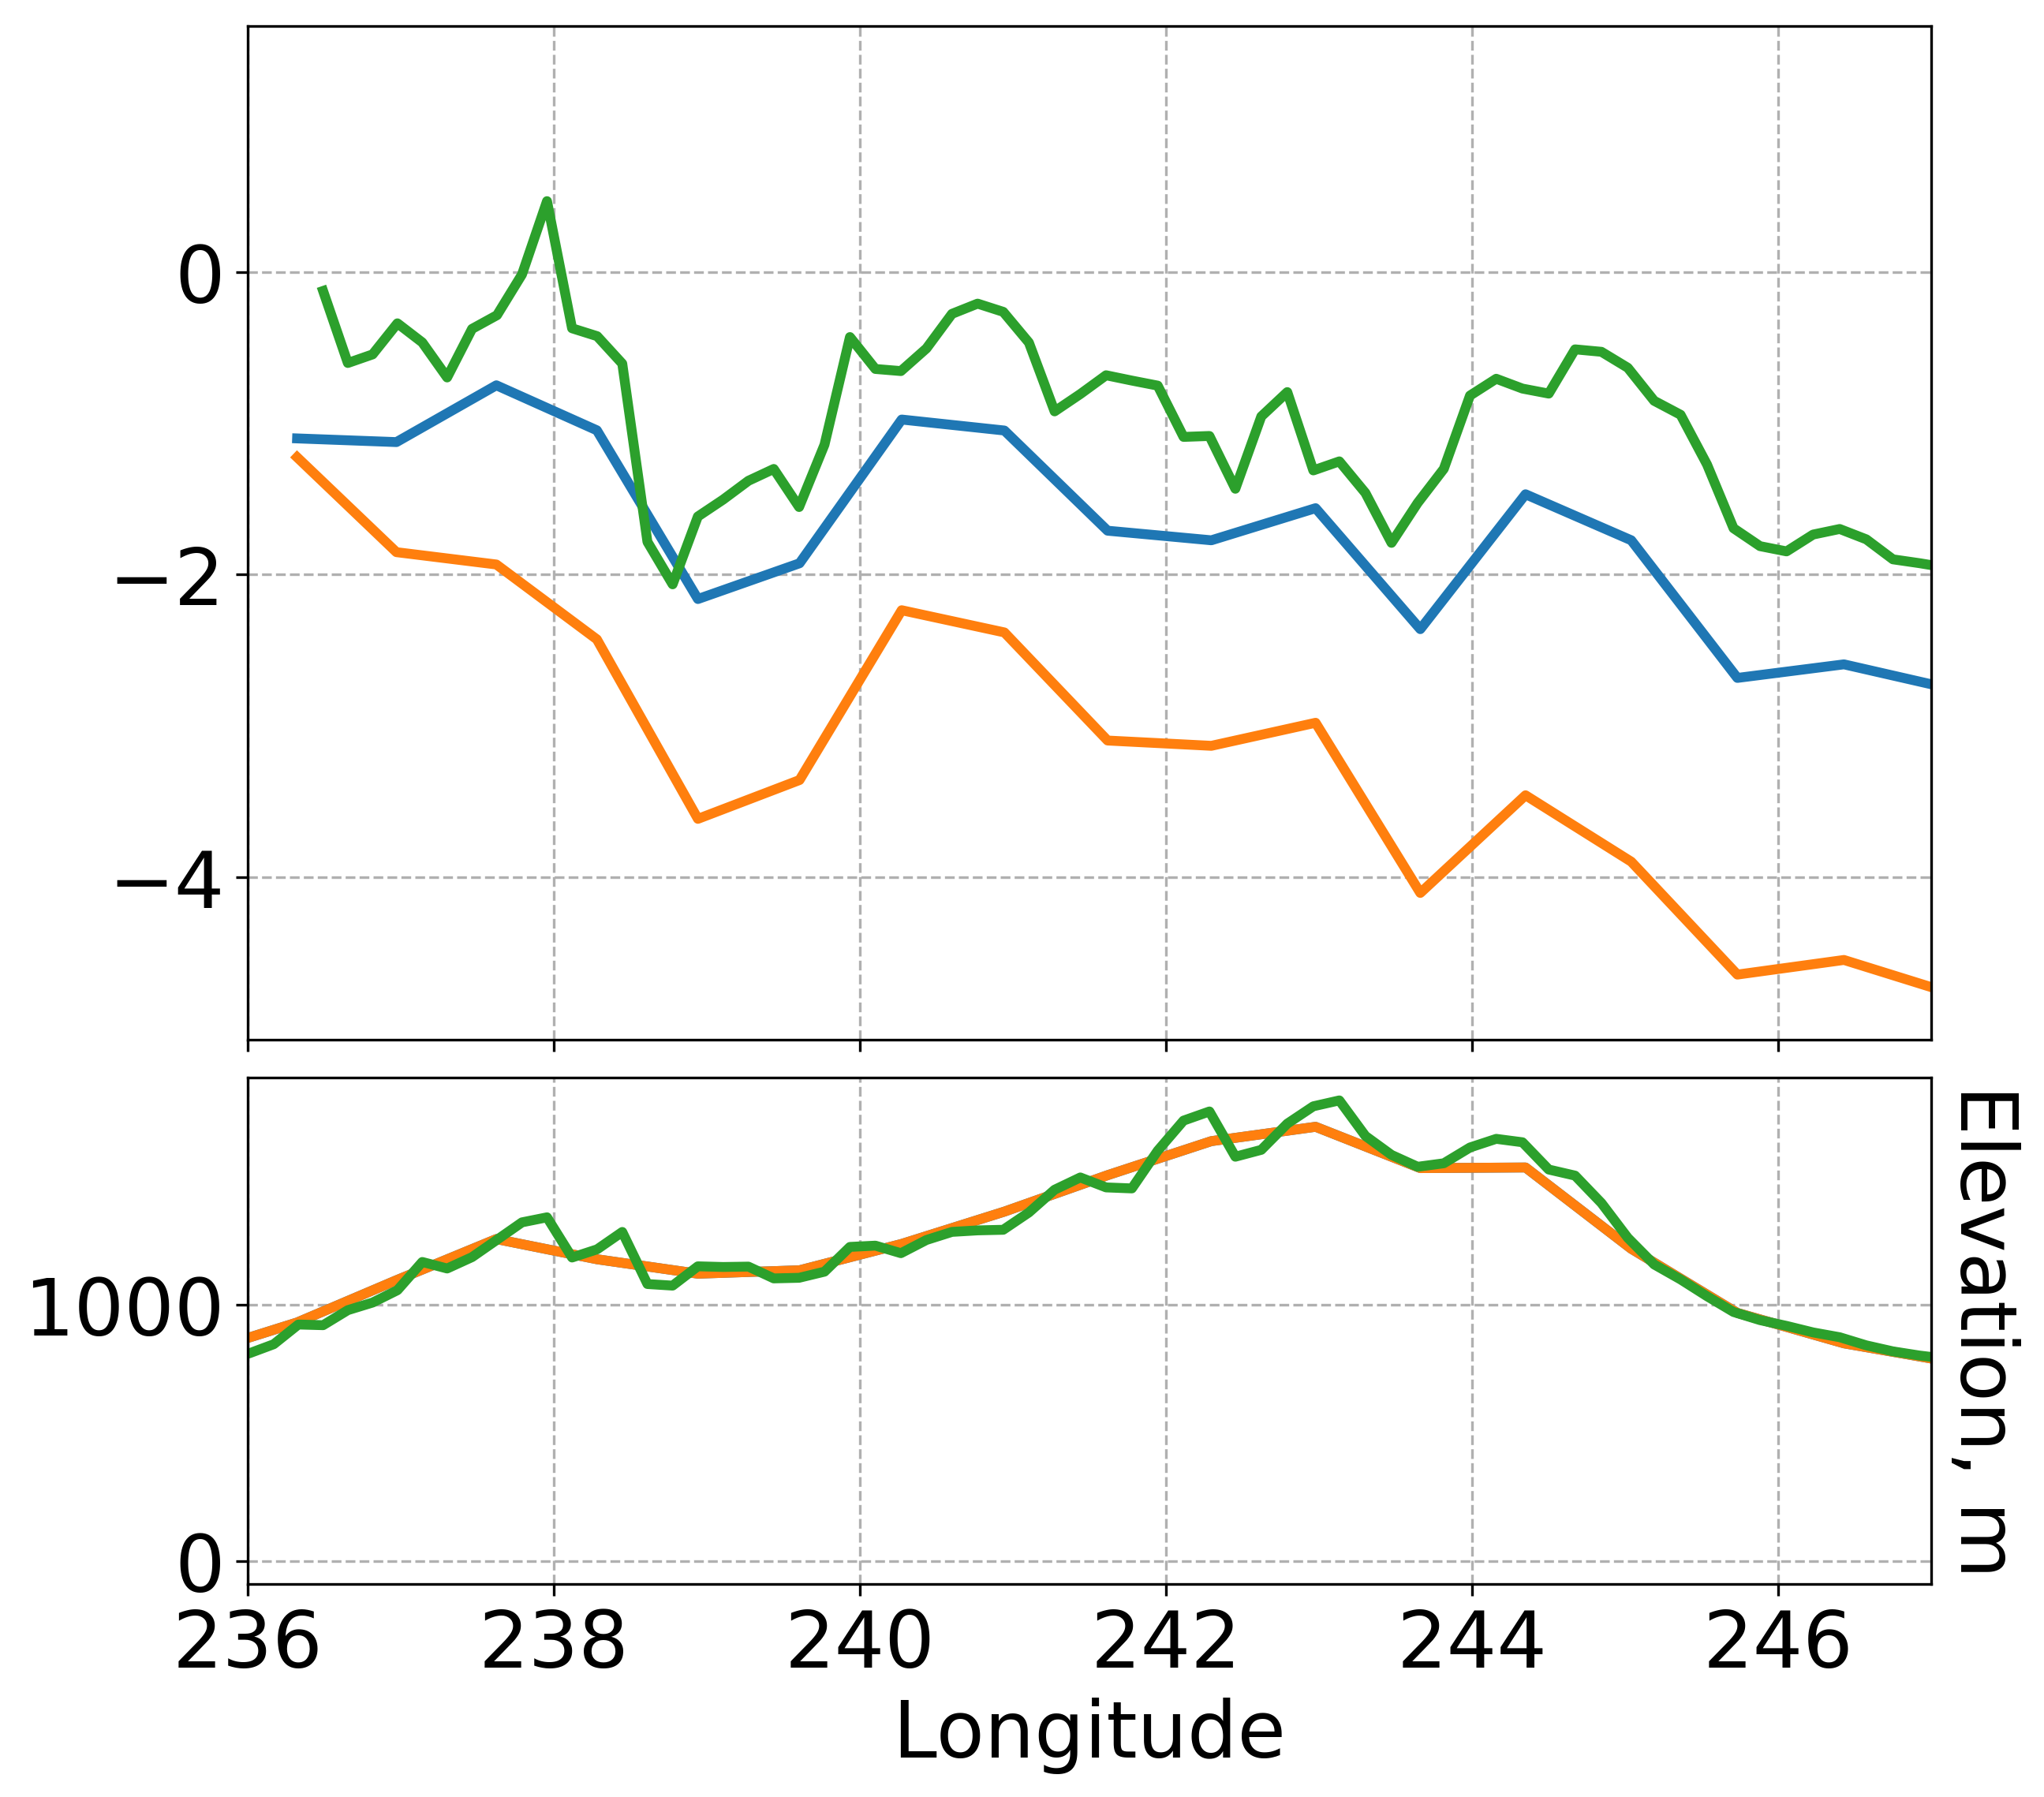
\includegraphics[width=0.31\linewidth, trim={0 8cm 0 0cm}, clip]{figures/meridional_avg/MAM_t_air_2m_daily_min}
    };

    \node[below=\hspc of tn90_mam] (tn90_jja) {
      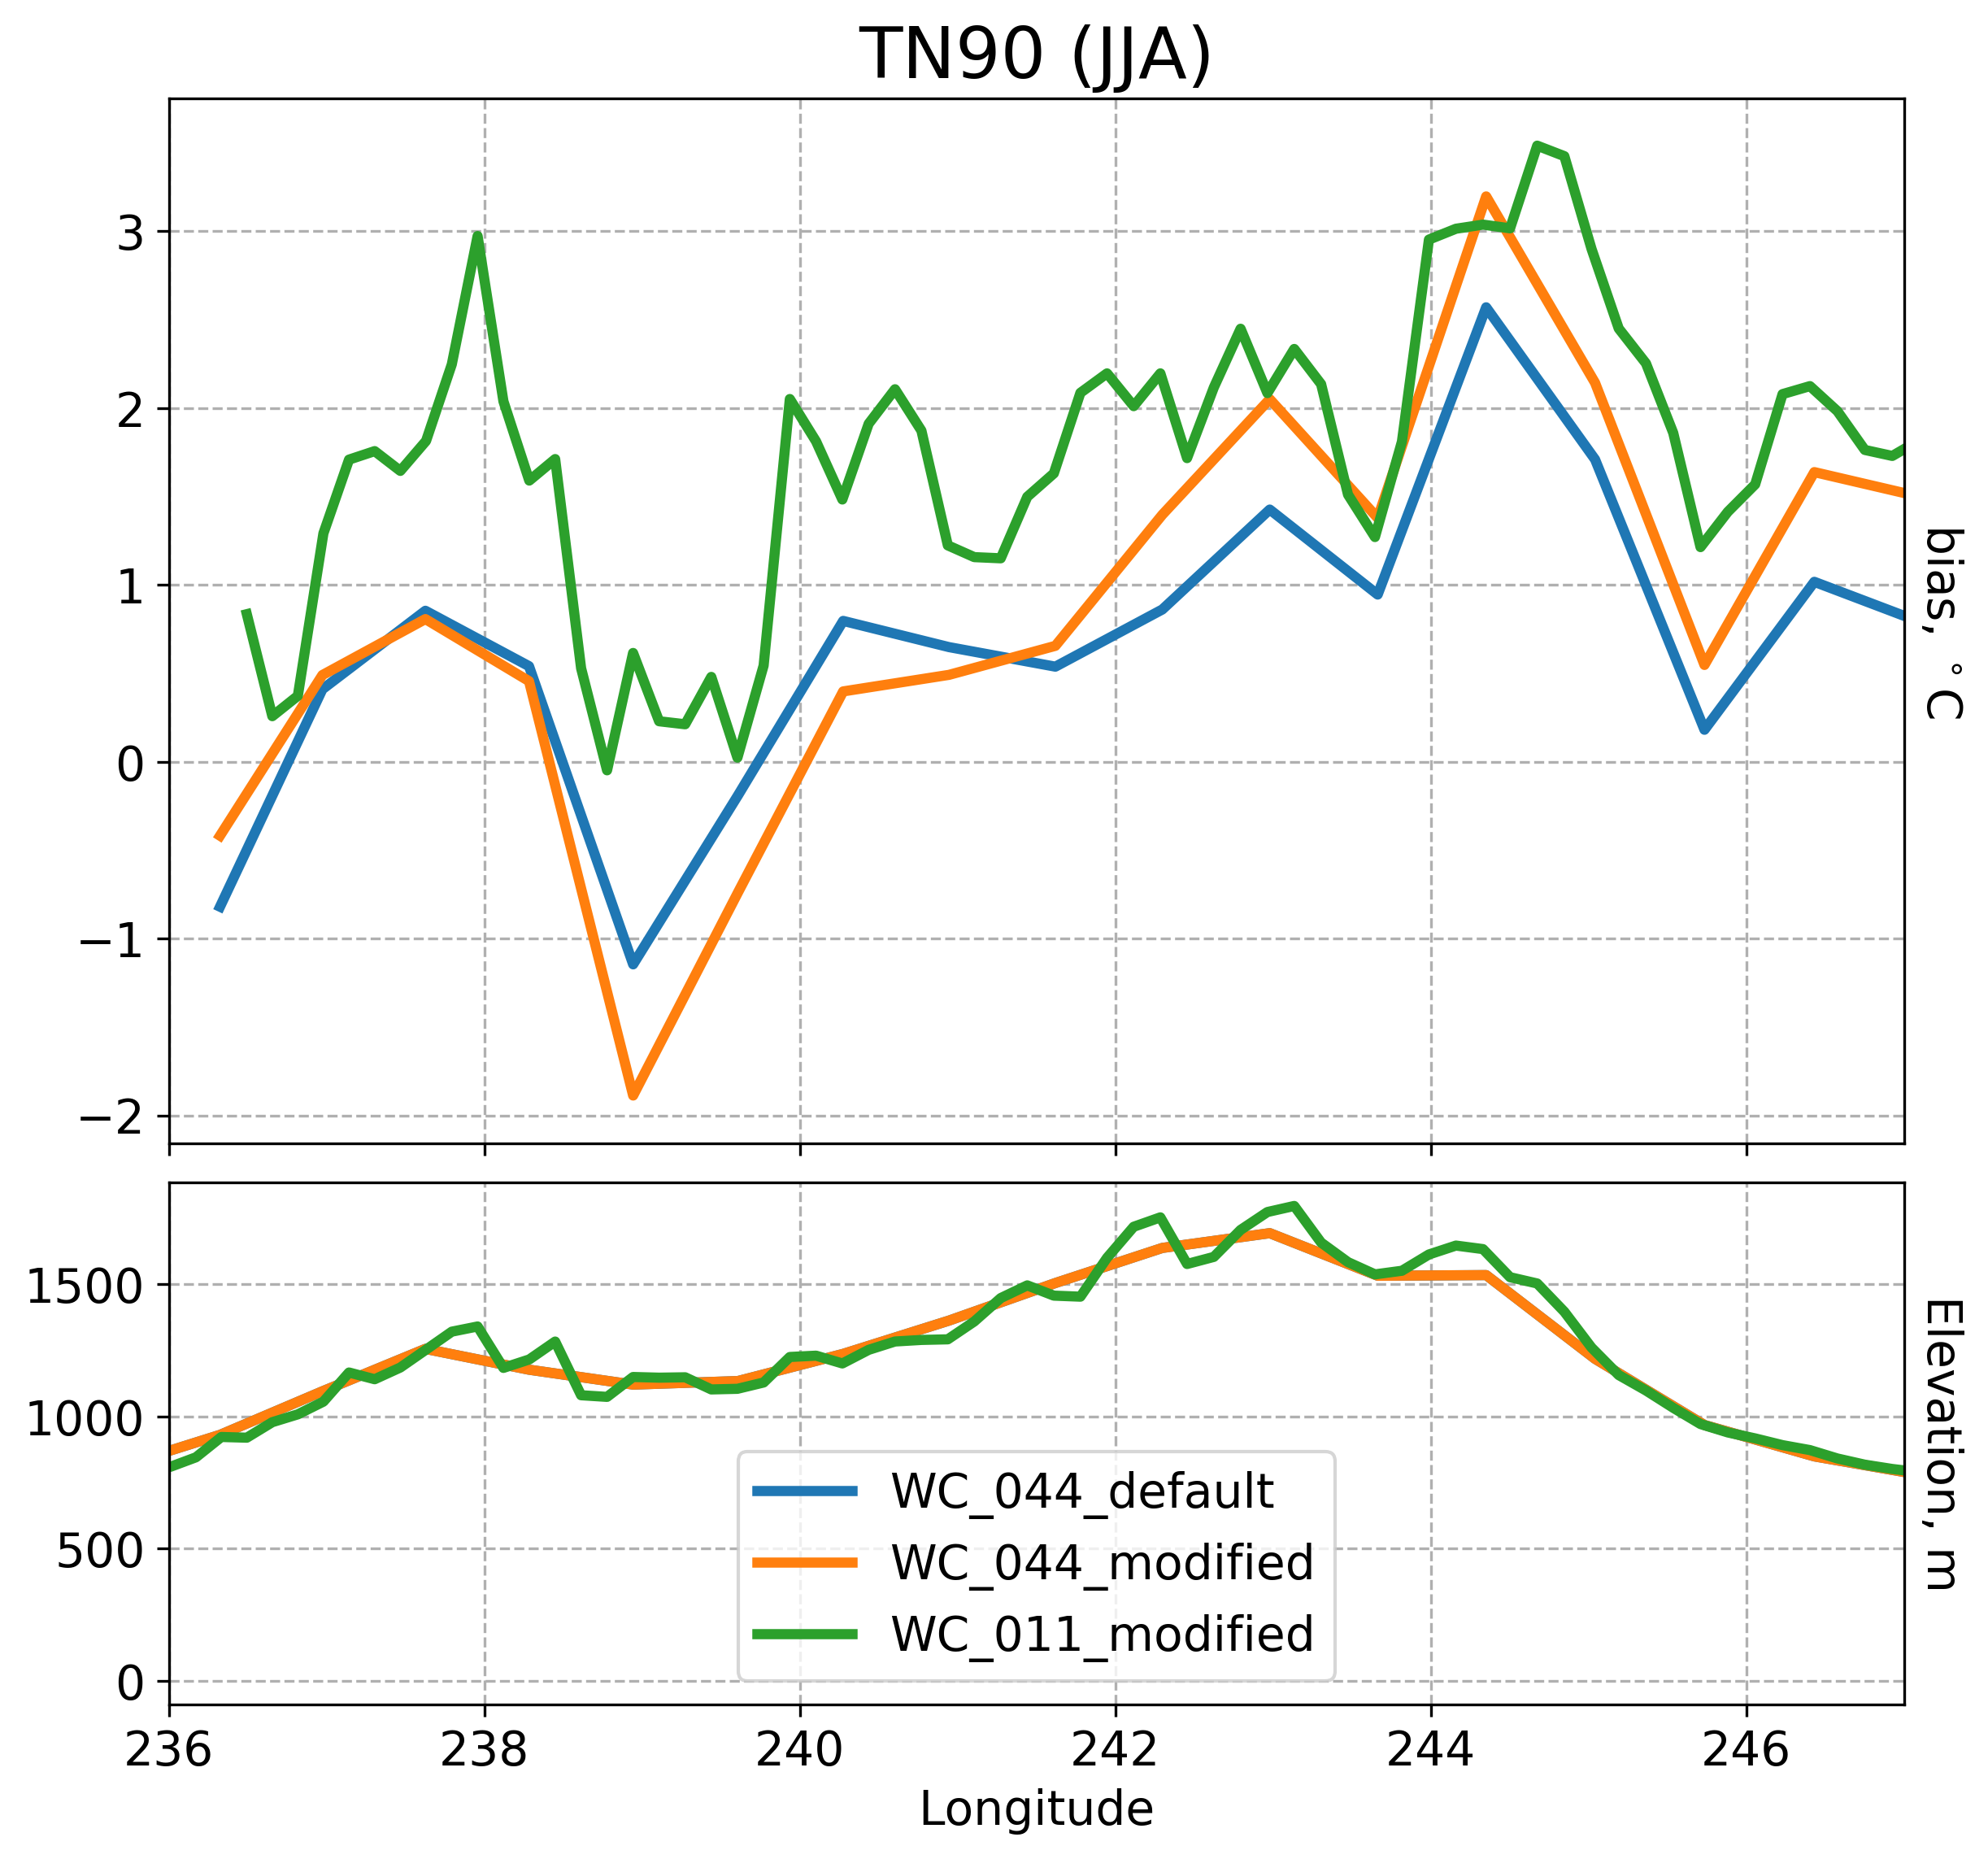
\includegraphics[width=0.31\linewidth, trim={0 8cm 0 0cm}, clip]{figures/meridional_avg/JJA_t_air_2m_daily_min}
    };

    \node[below=\hspc of tn90_jja] (tn90_son) {
      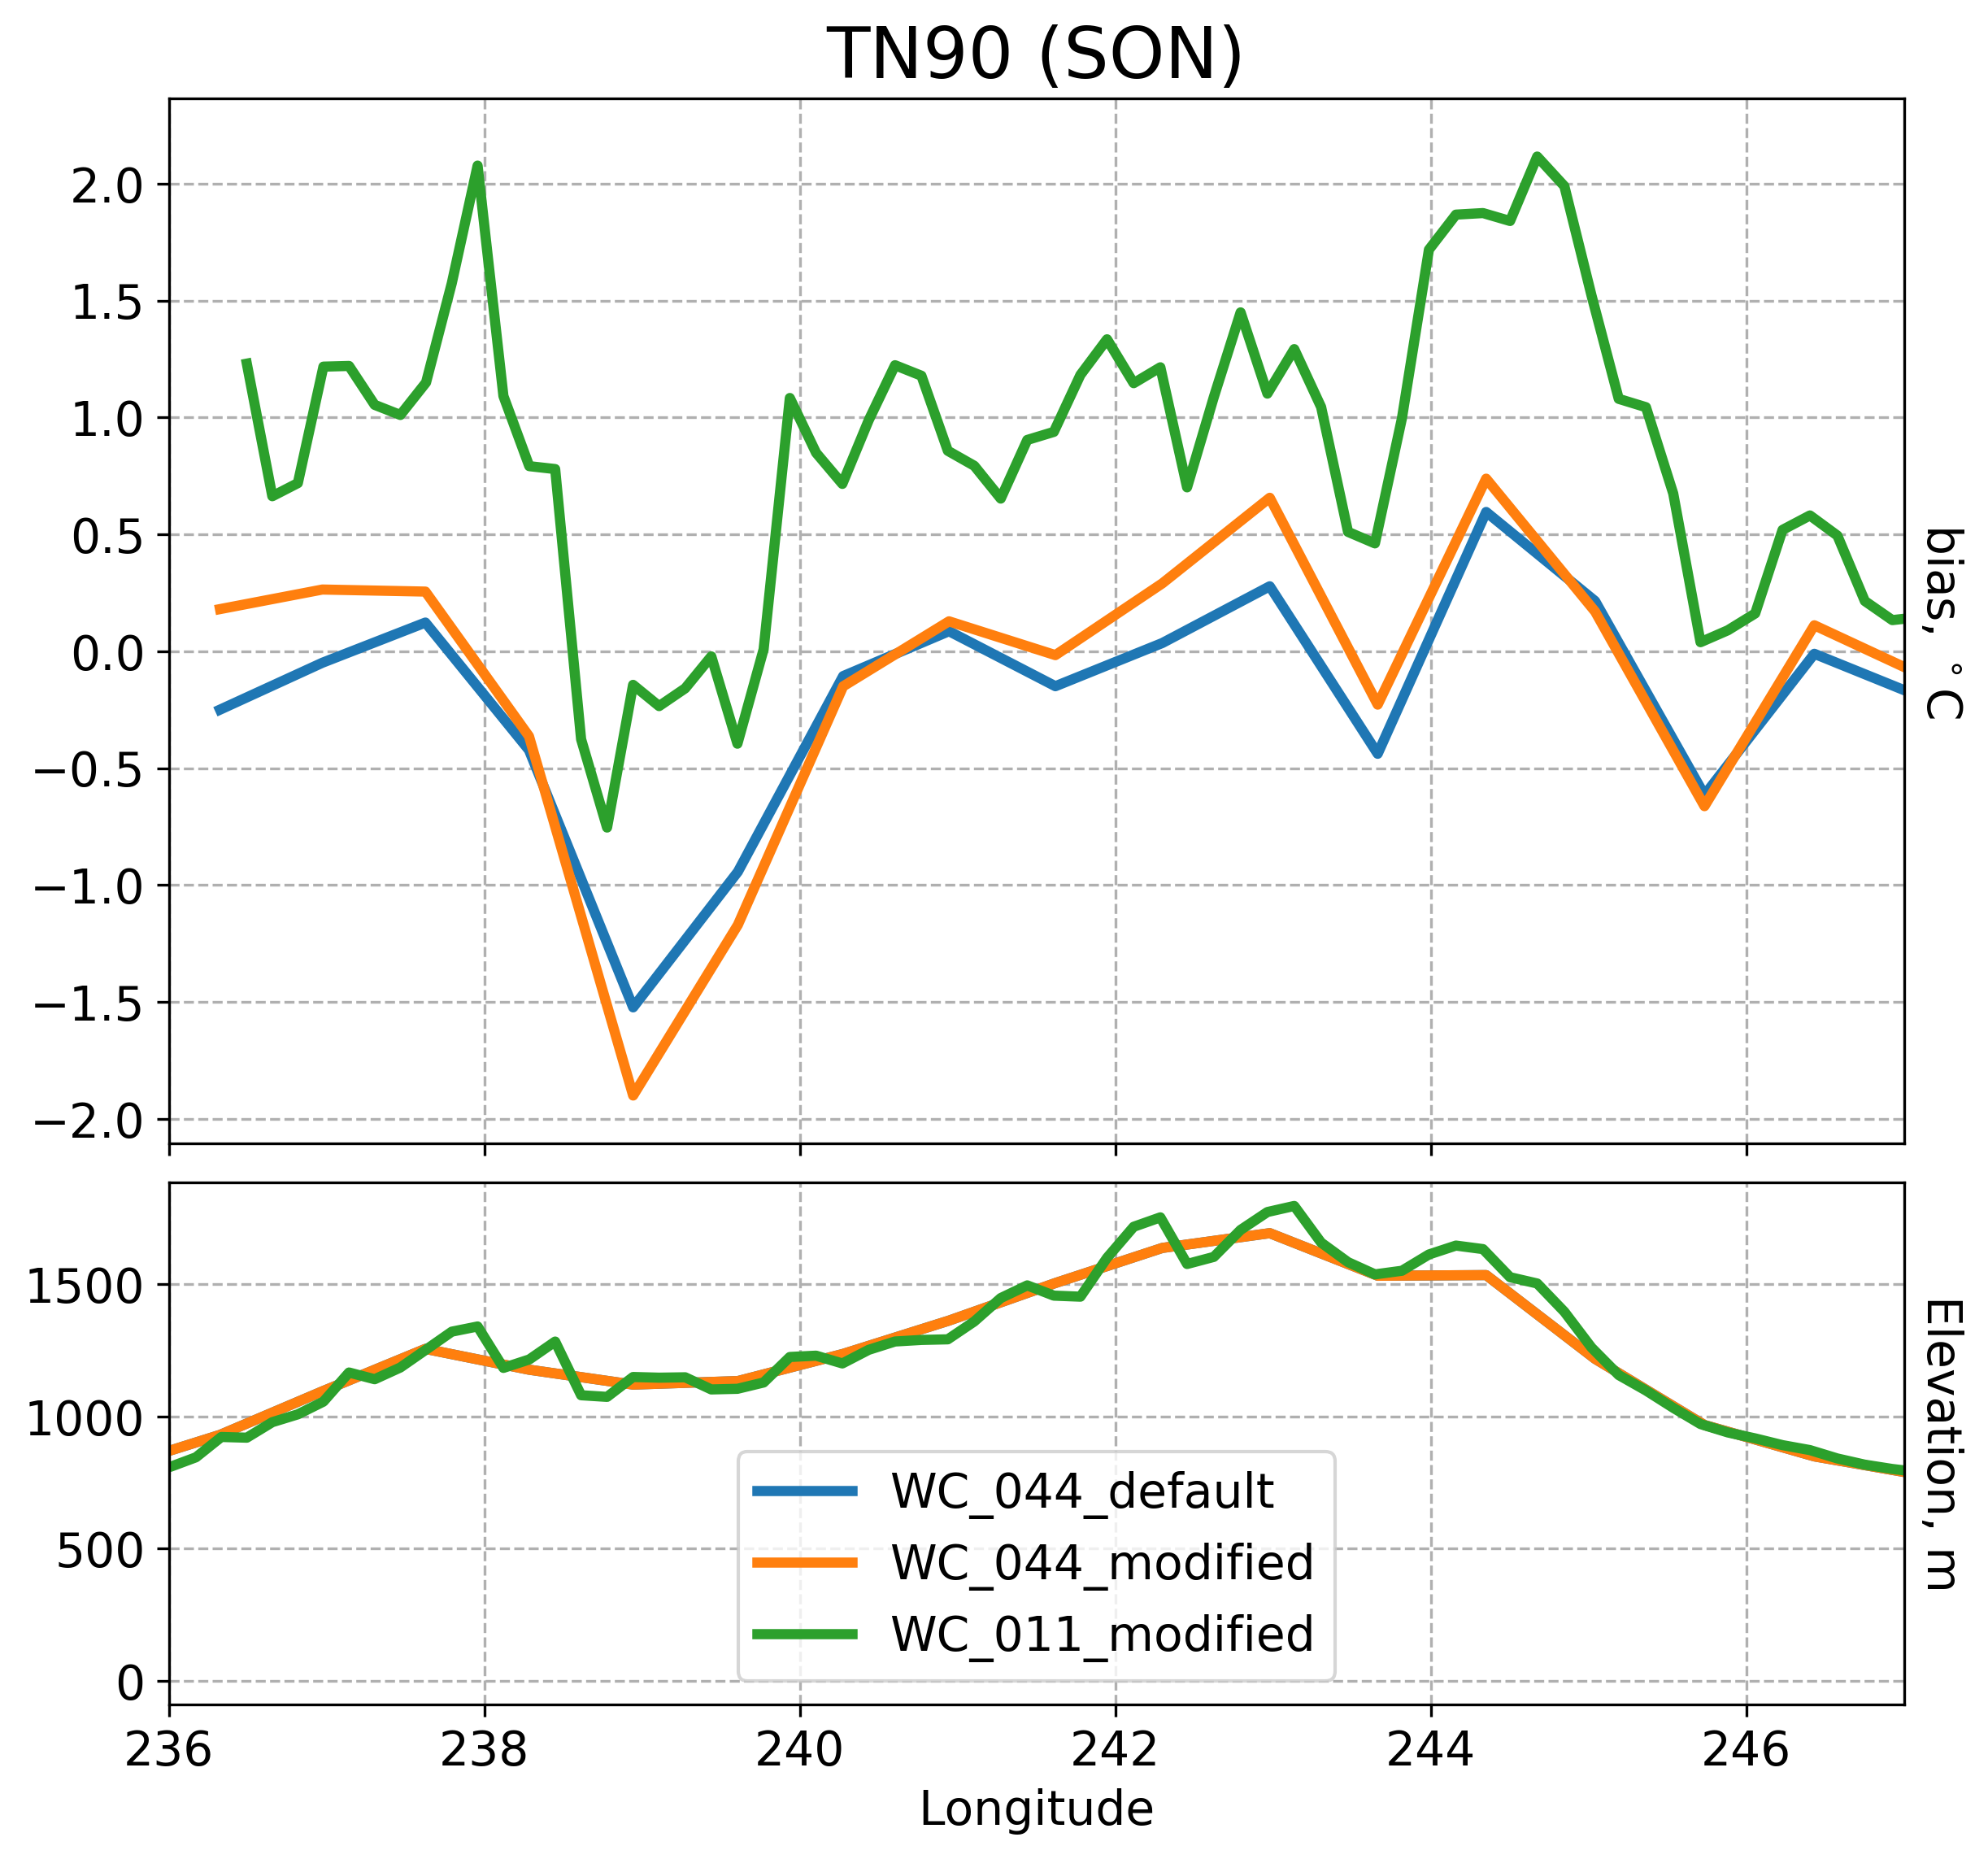
\includegraphics[width=0.31\linewidth, trim={0 0cm 0 0cm}, clip]{figures/meridional_avg/SON_t_air_2m_daily_min}
    };

    %PR90
    \node[label={\small PR90}, right=\wspc of tn90_djf] (pr90_djf) {
      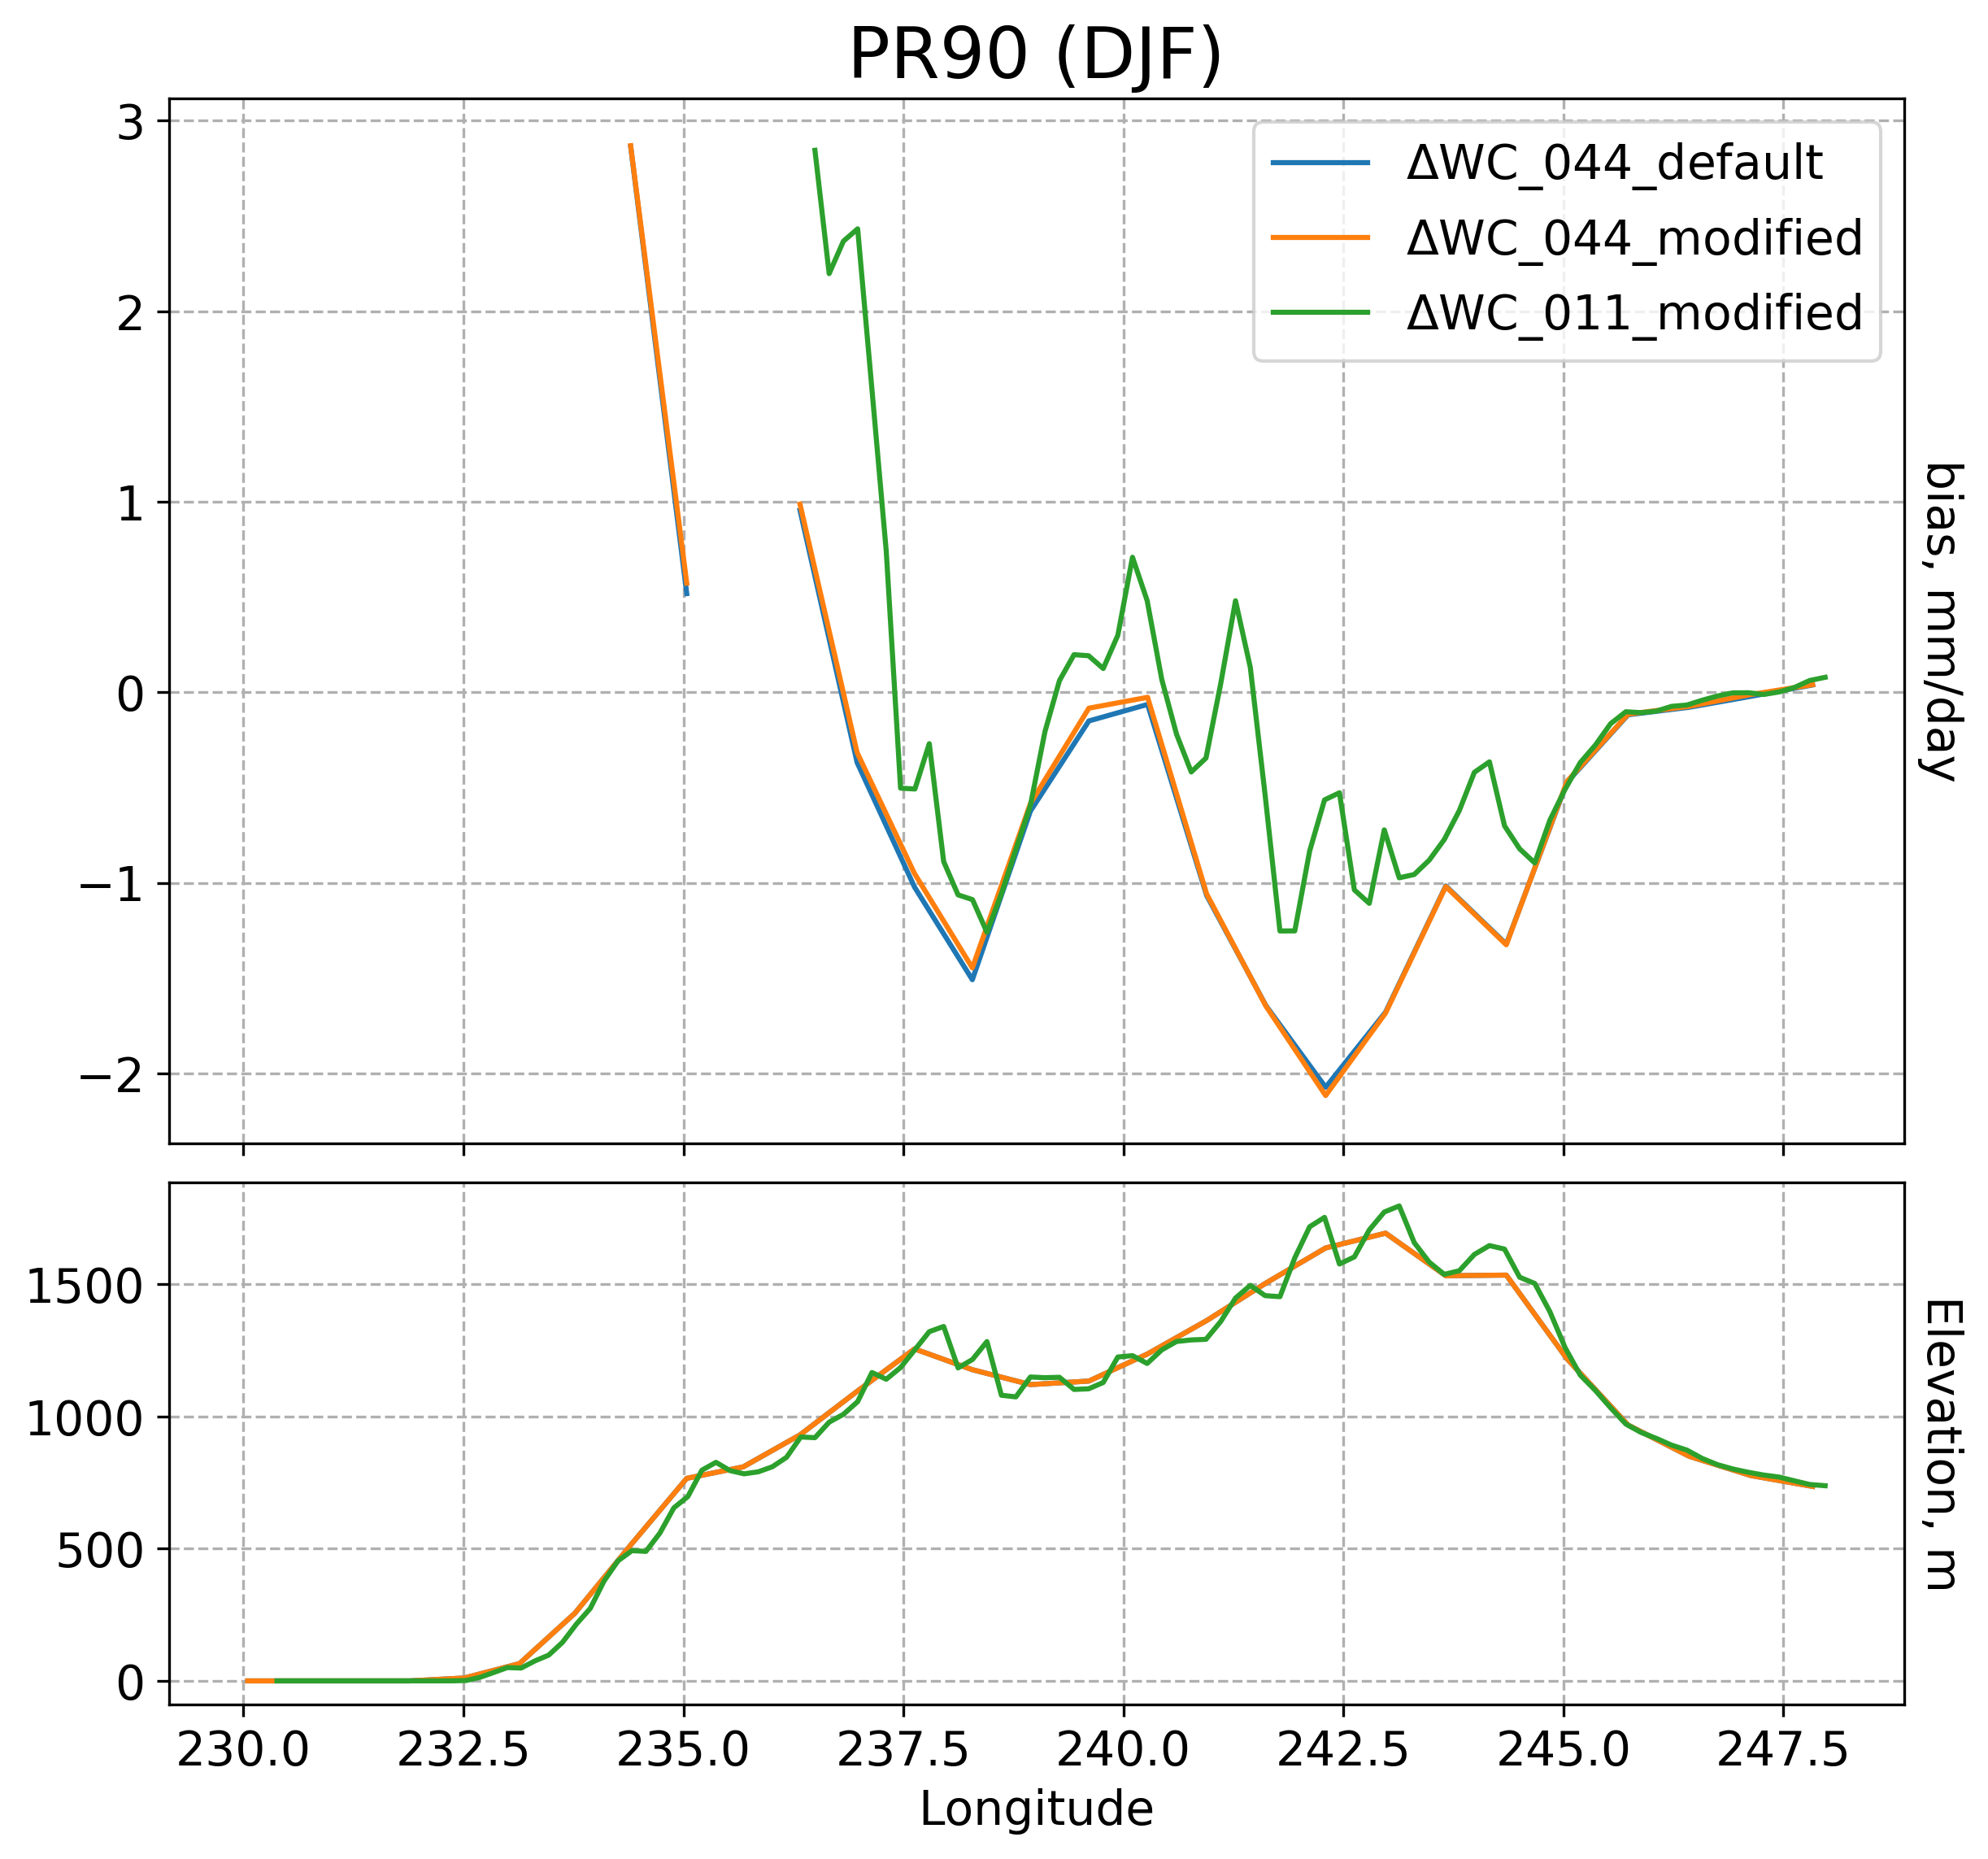
\includegraphics[width=0.31\linewidth, trim={0 8cm 0 0cm}, clip]{figures/meridional_avg/DJF_total_prec}
    };

    \node[below=\hspc of pr90_djf] (pr90_mam) {
      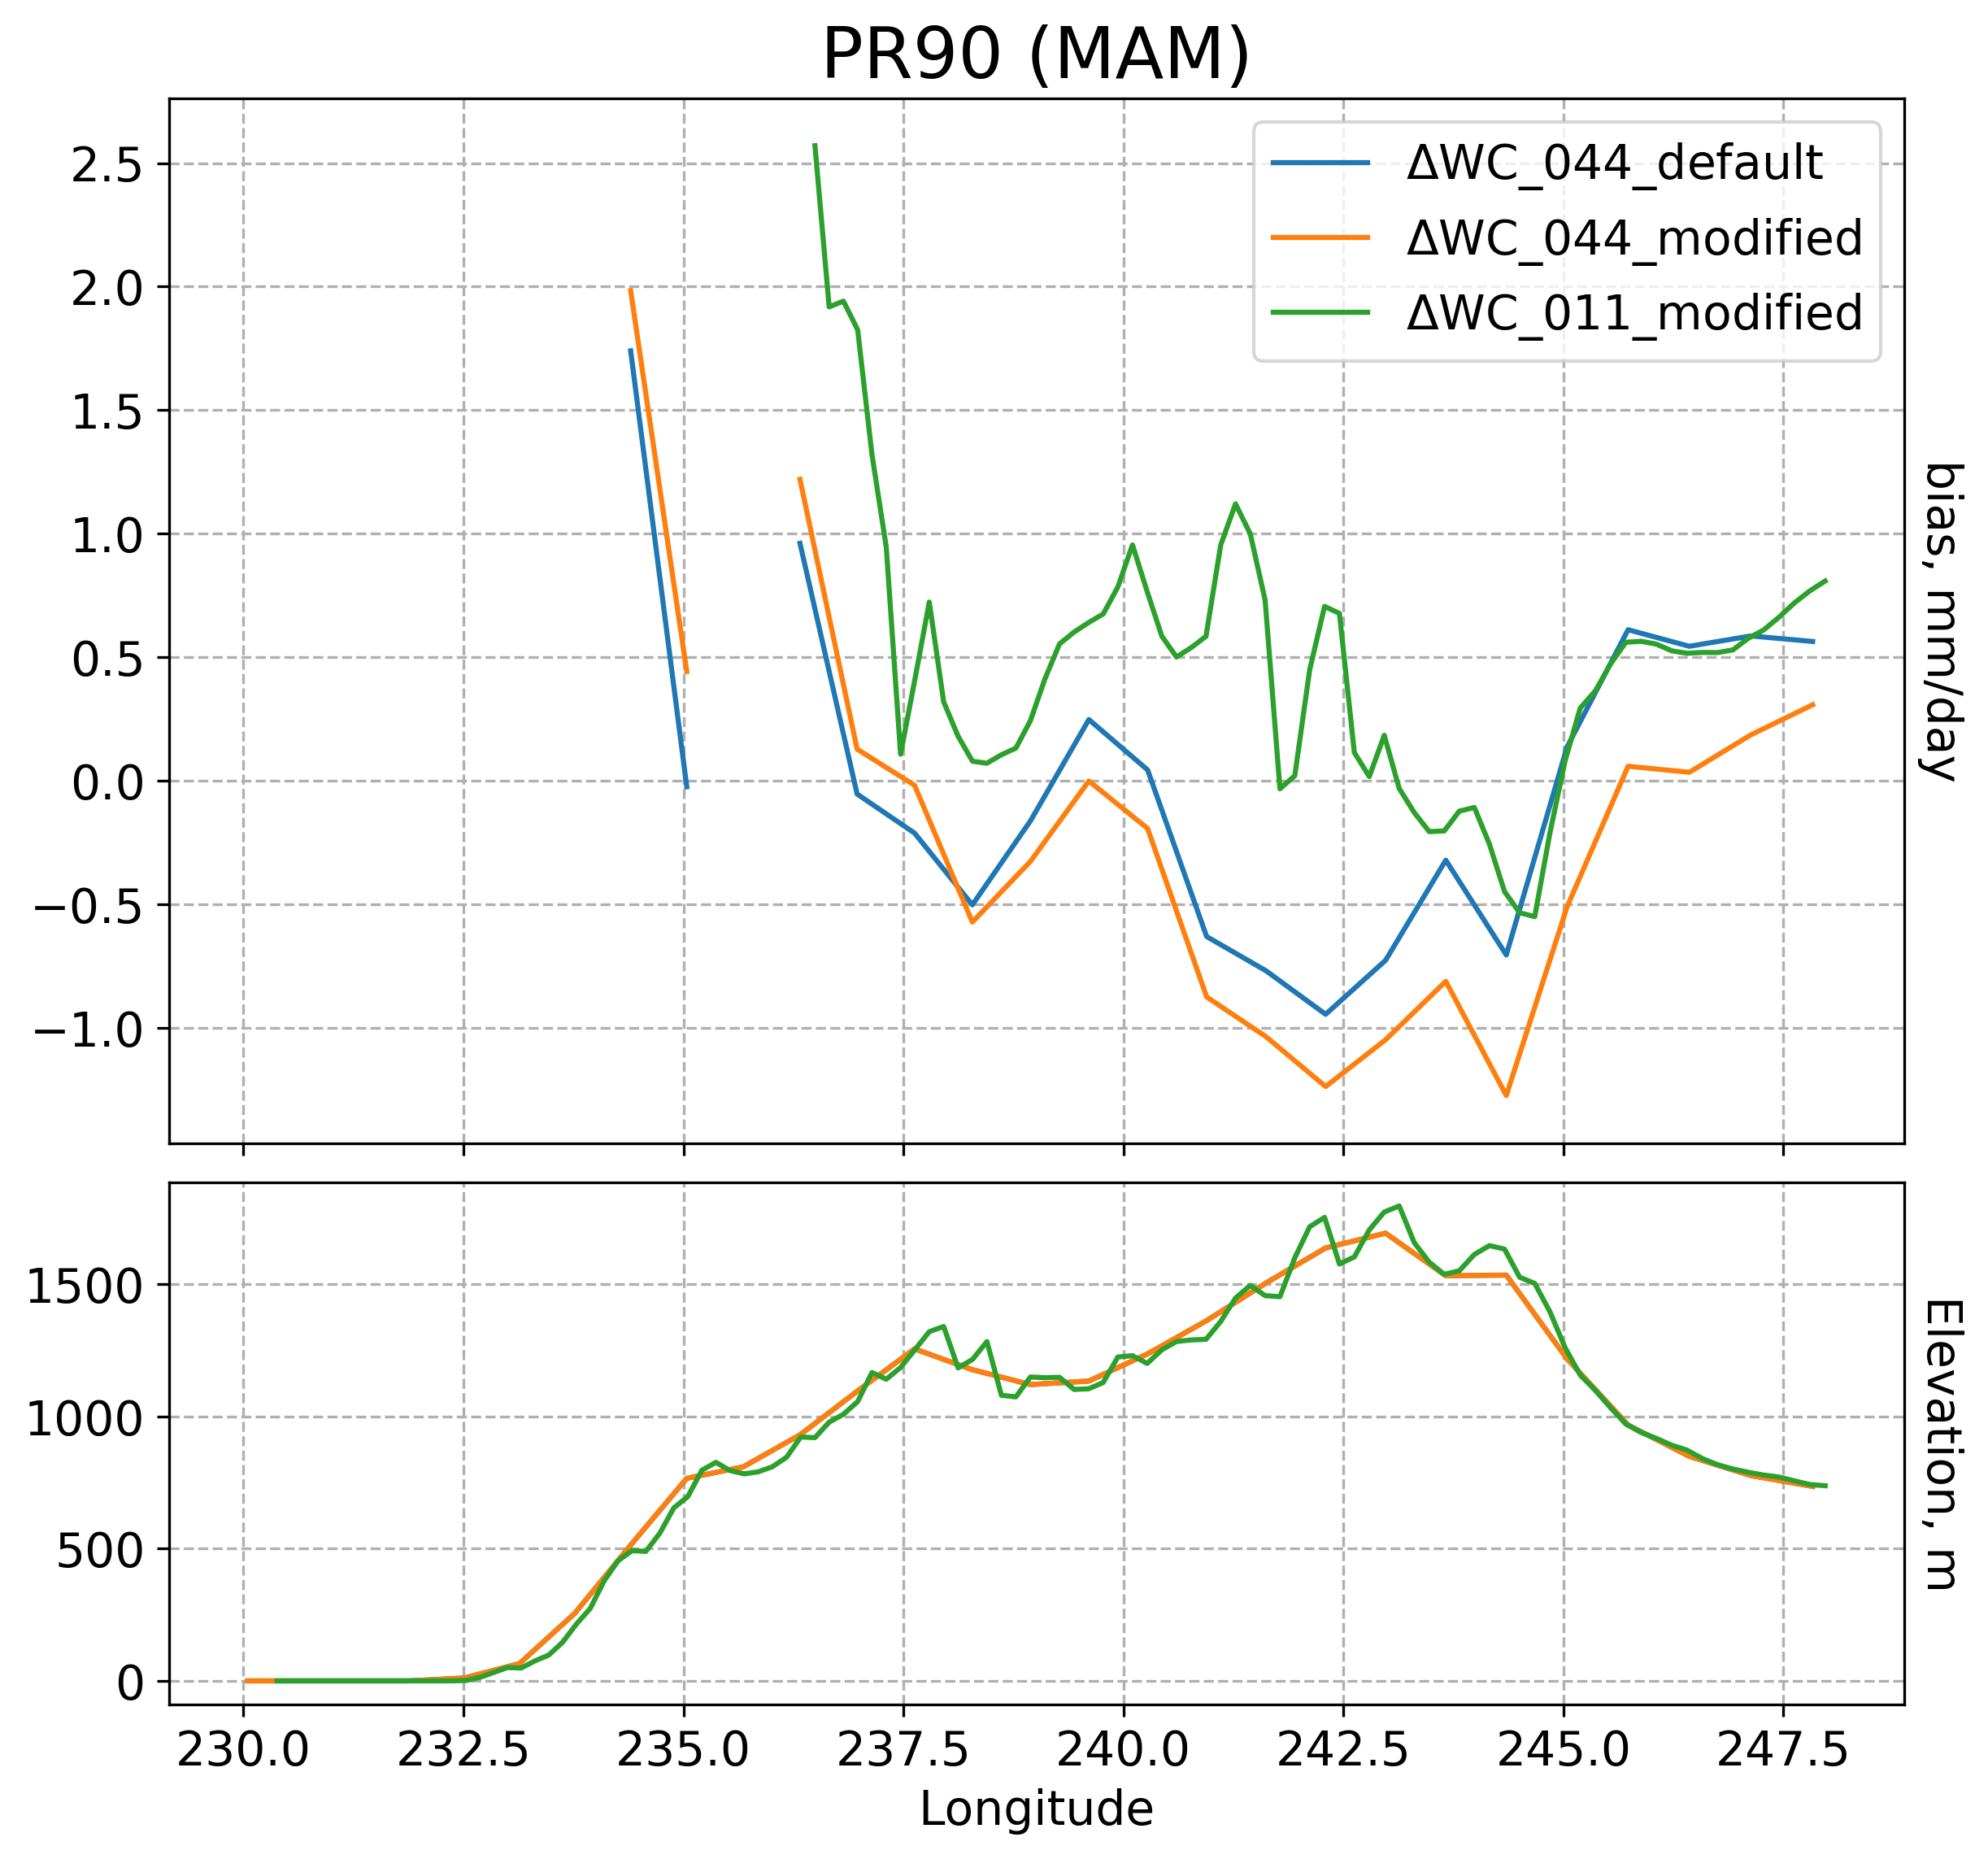
\includegraphics[width=0.31\linewidth, trim={0 8cm 0 0cm}, clip]{figures/meridional_avg/MAM_total_prec}
    };

    \node[below=\hspc of pr90_mam] (pr90_jja) {
      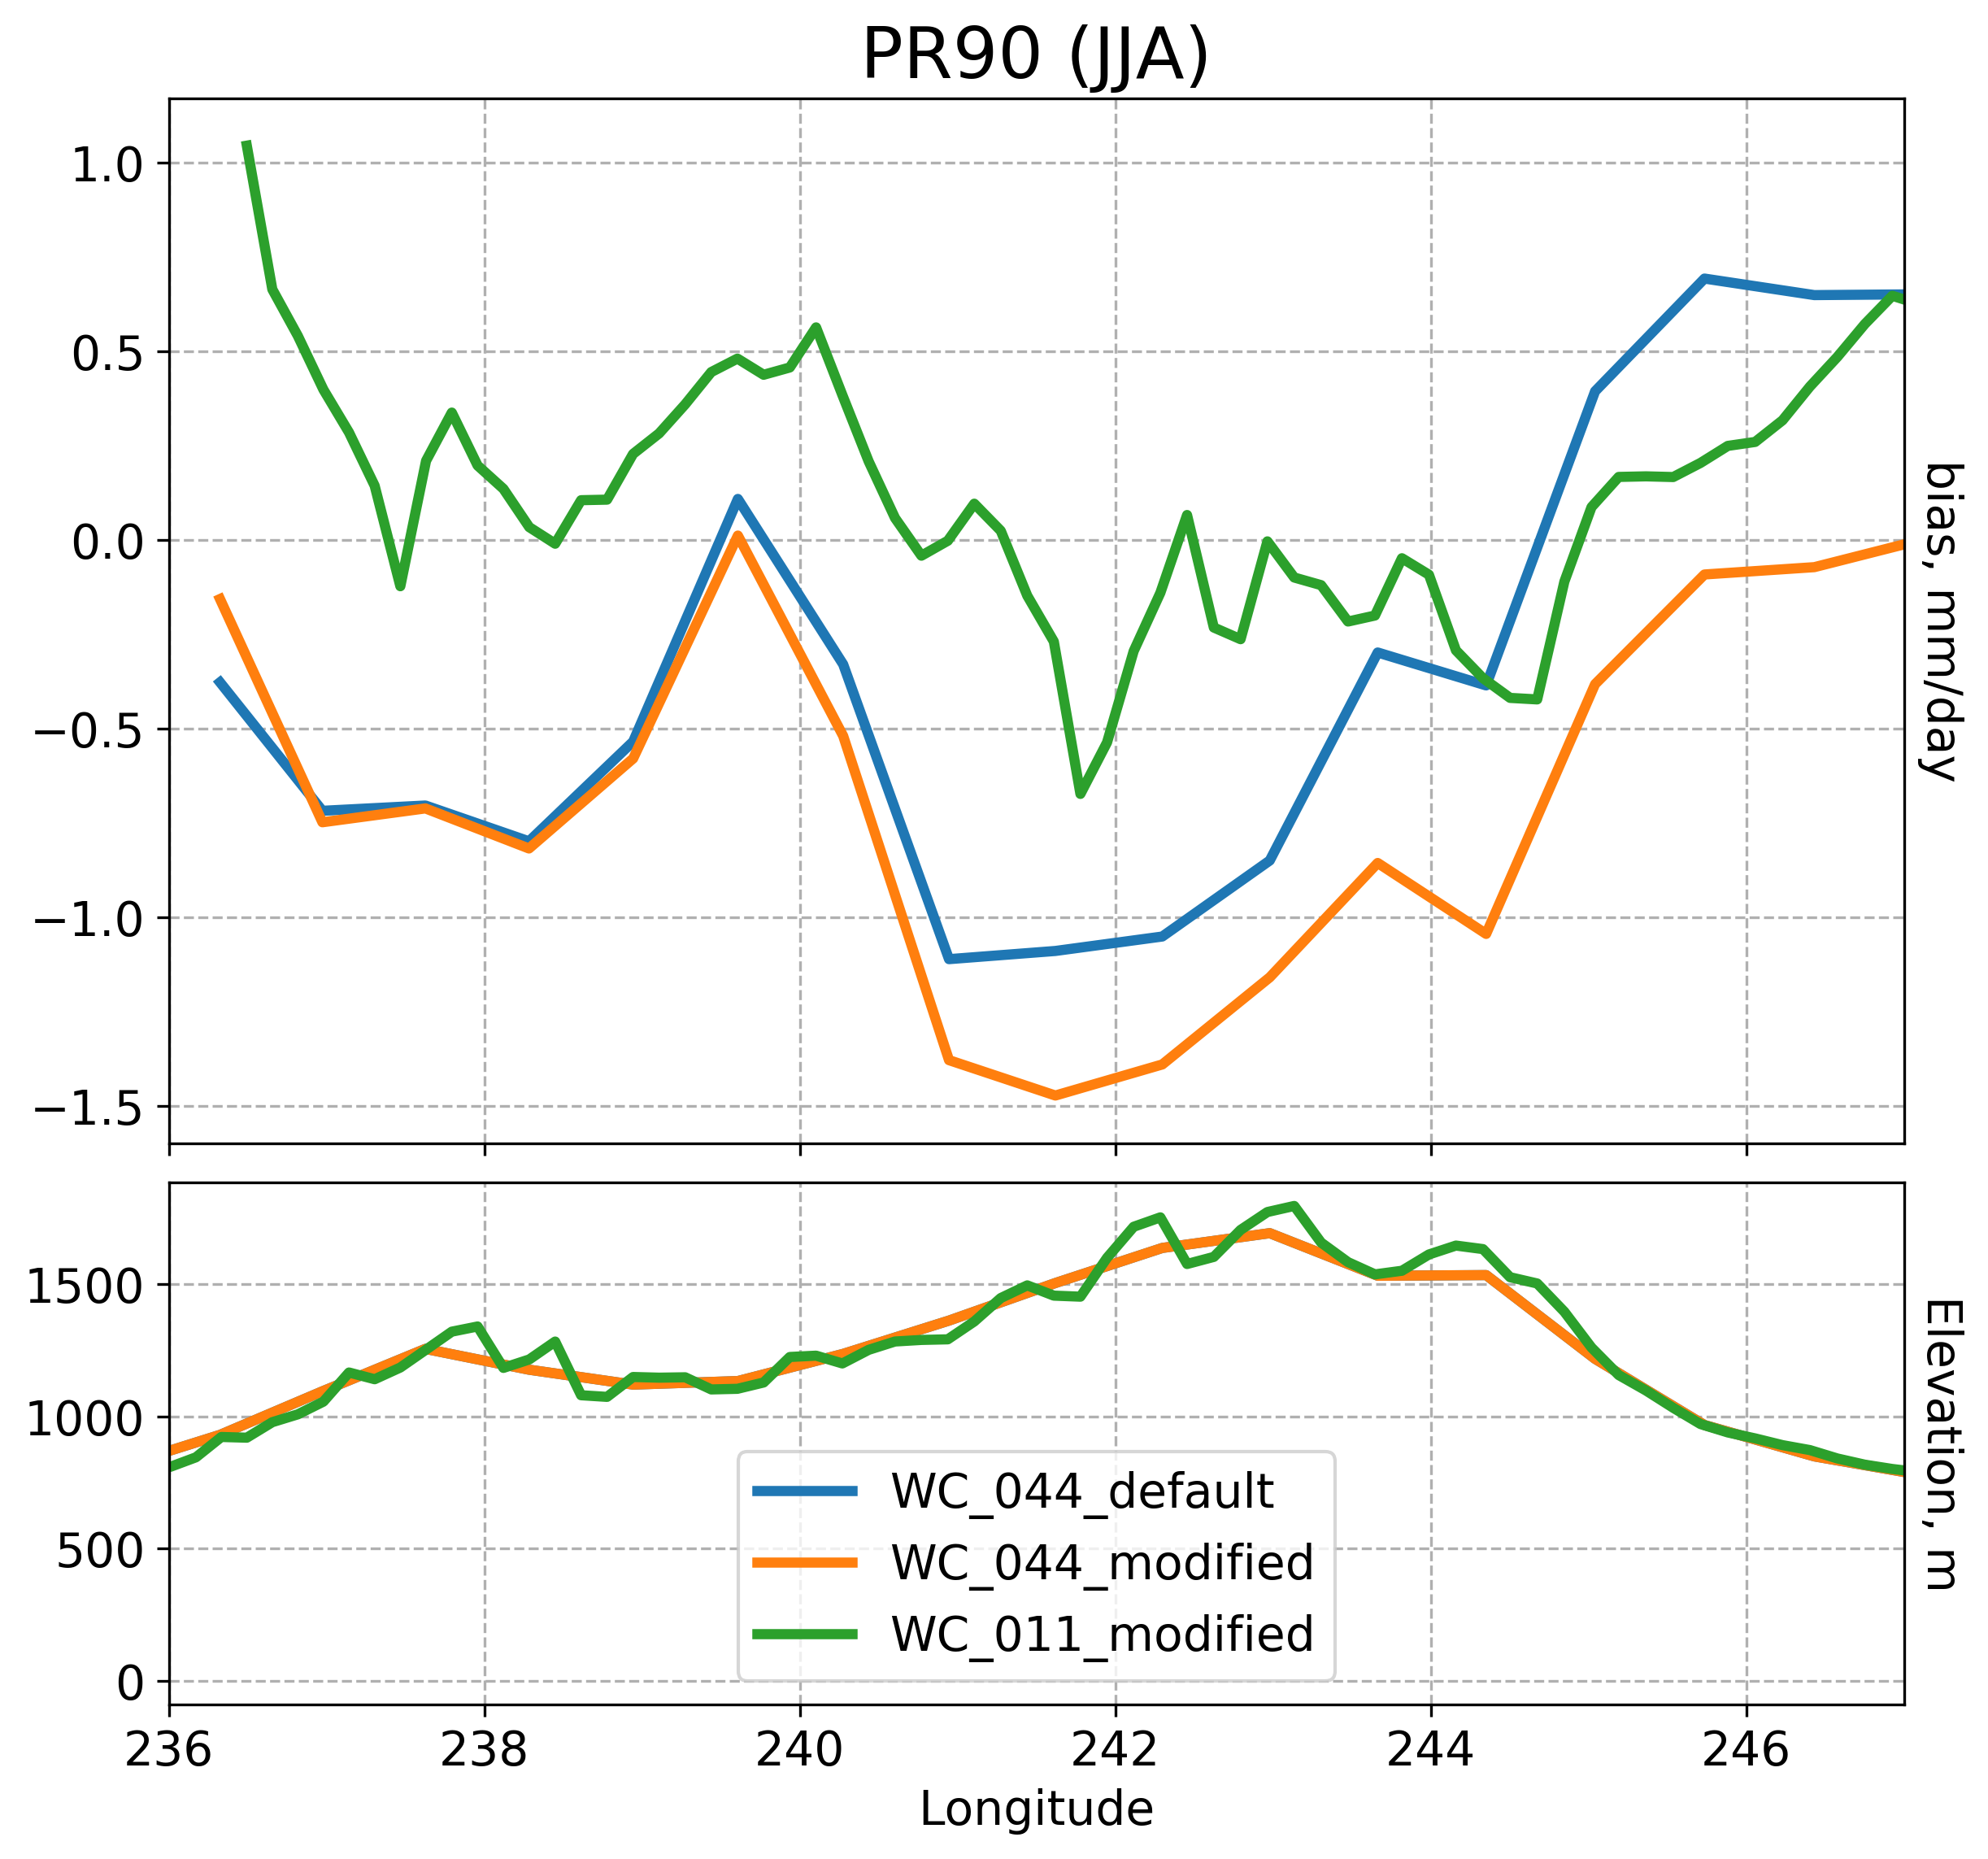
\includegraphics[width=0.31\linewidth, trim={0 8cm 0 0cm}, clip]{figures/meridional_avg/JJA_total_prec}
    };

    \node[below=\hspc of pr90_jja] (pr90_son) {
      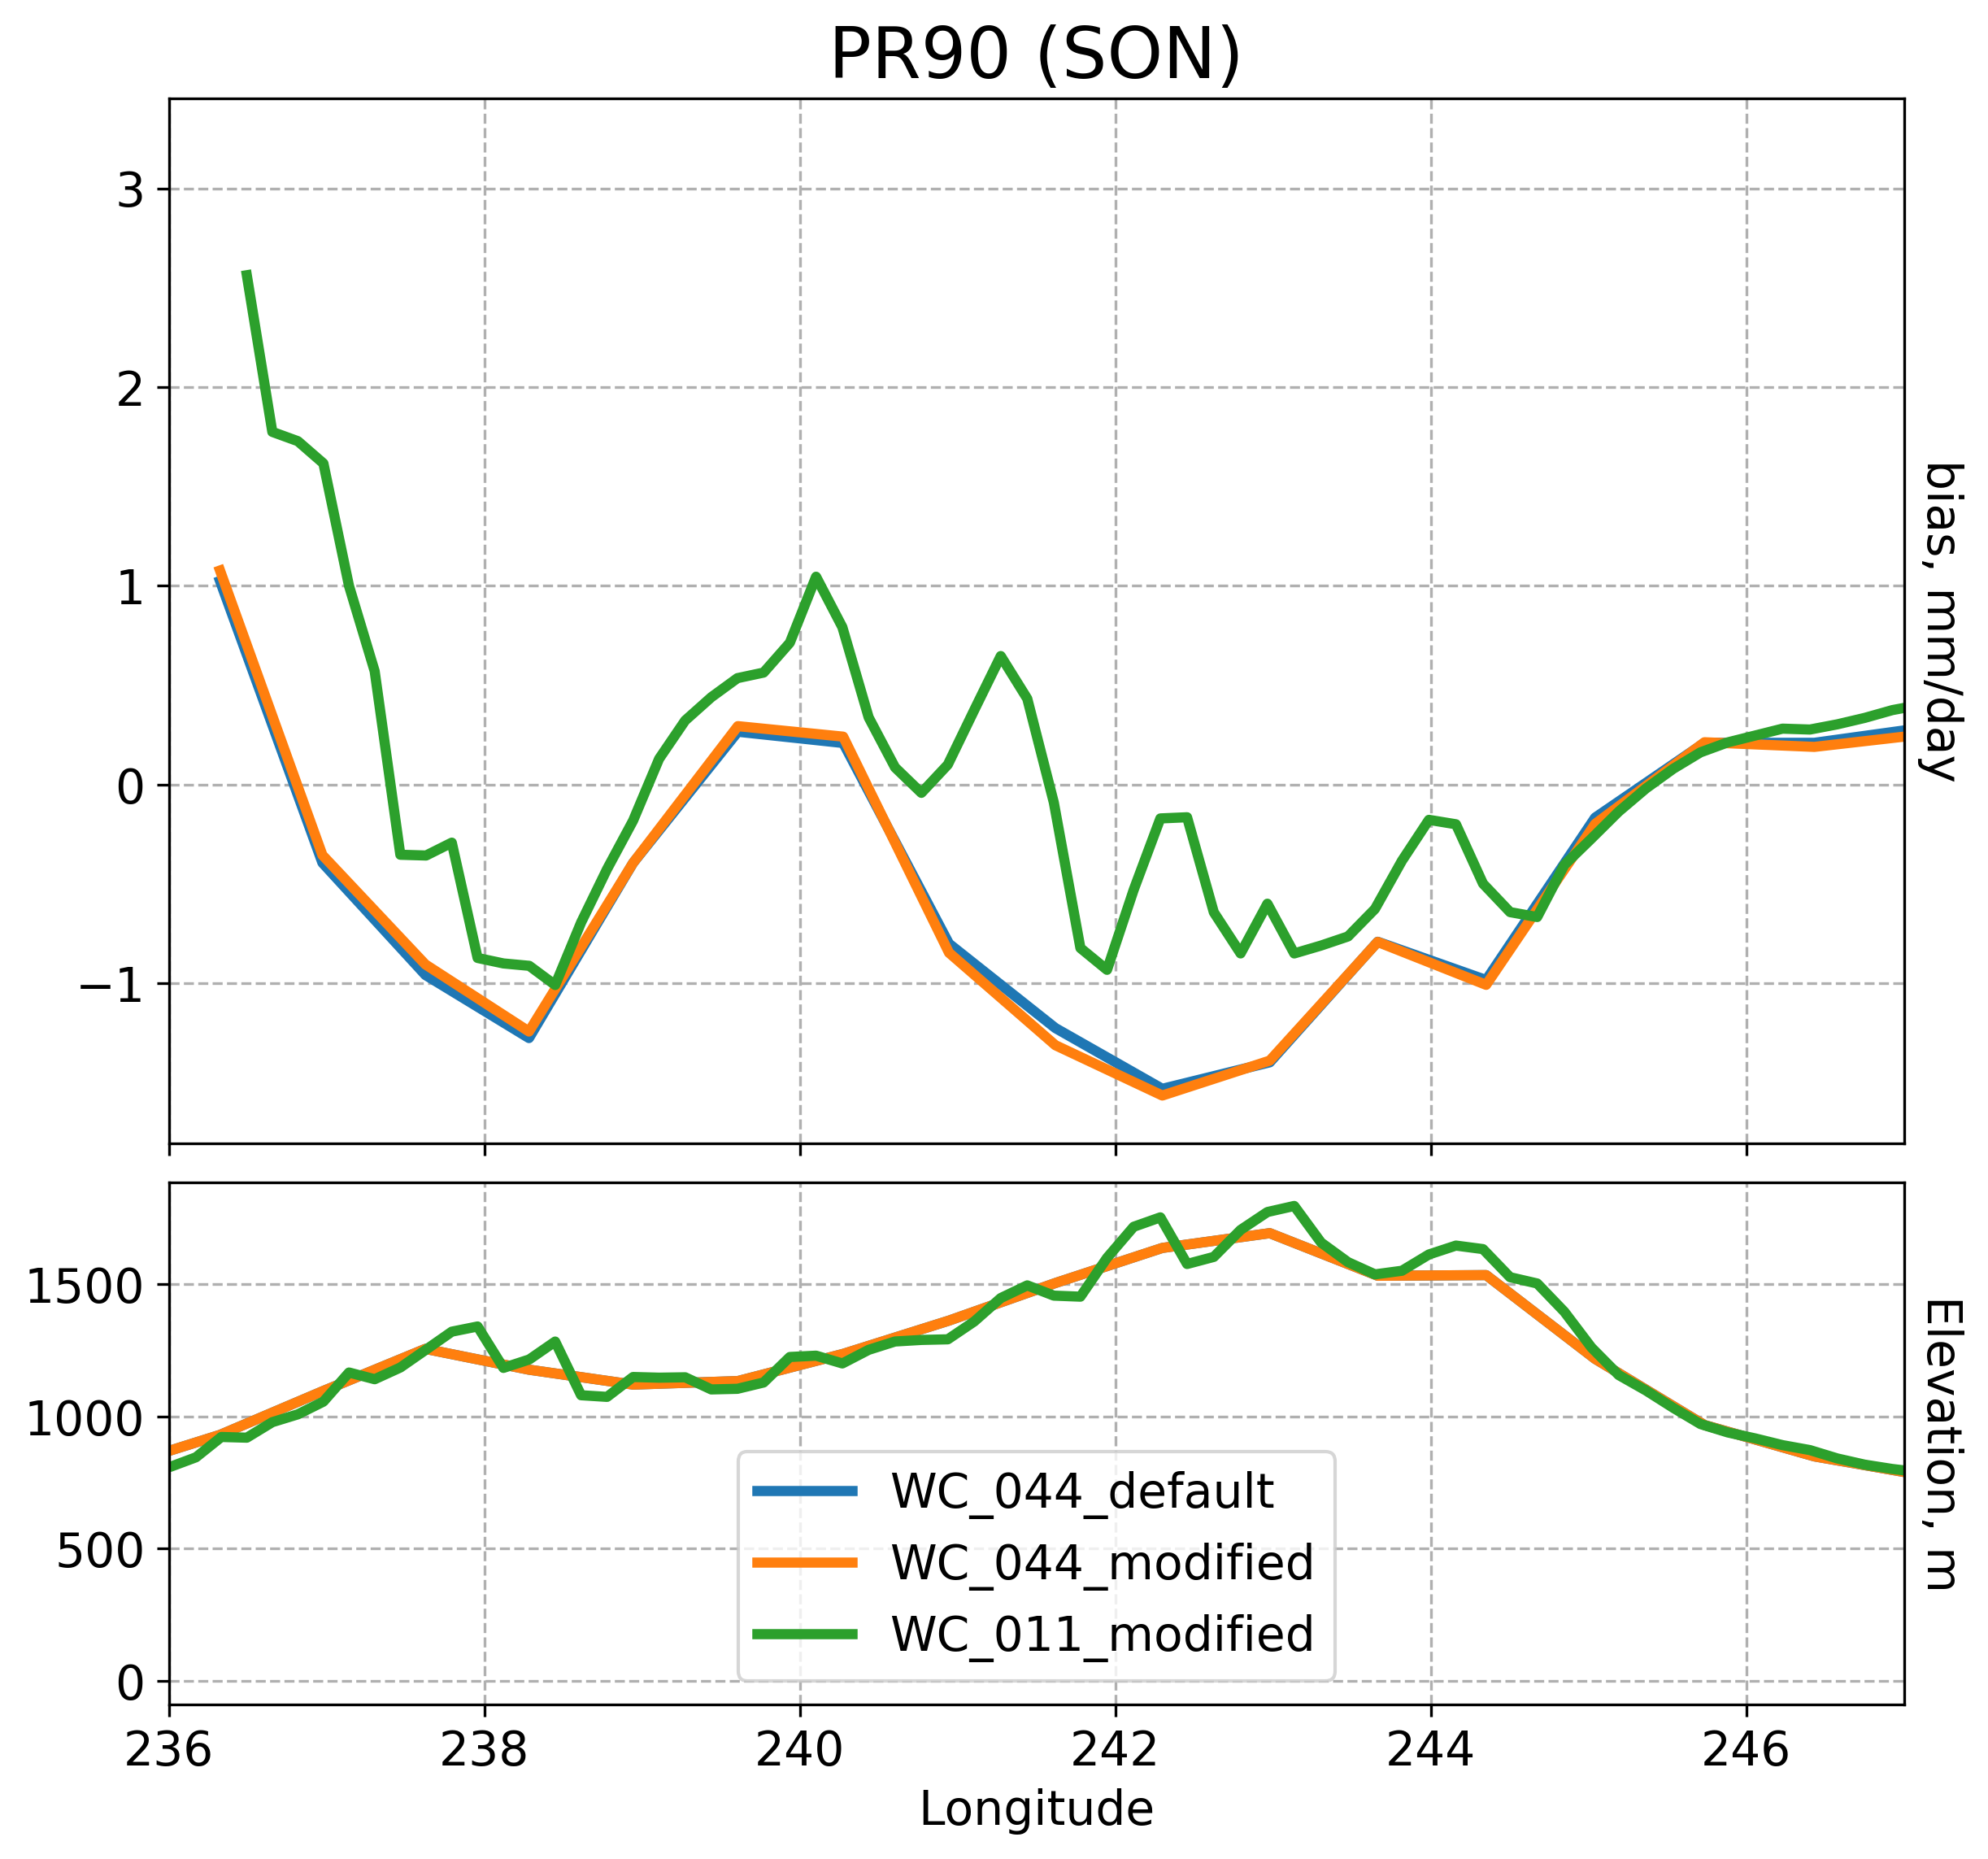
\includegraphics[width=0.31\linewidth, trim={0 0cm 0 0cm}, clip]{figures/meridional_avg/SON_total_prec}
    };


    %elevation
    % \node[below=\hspc of tx10_son] (el1) {
    %   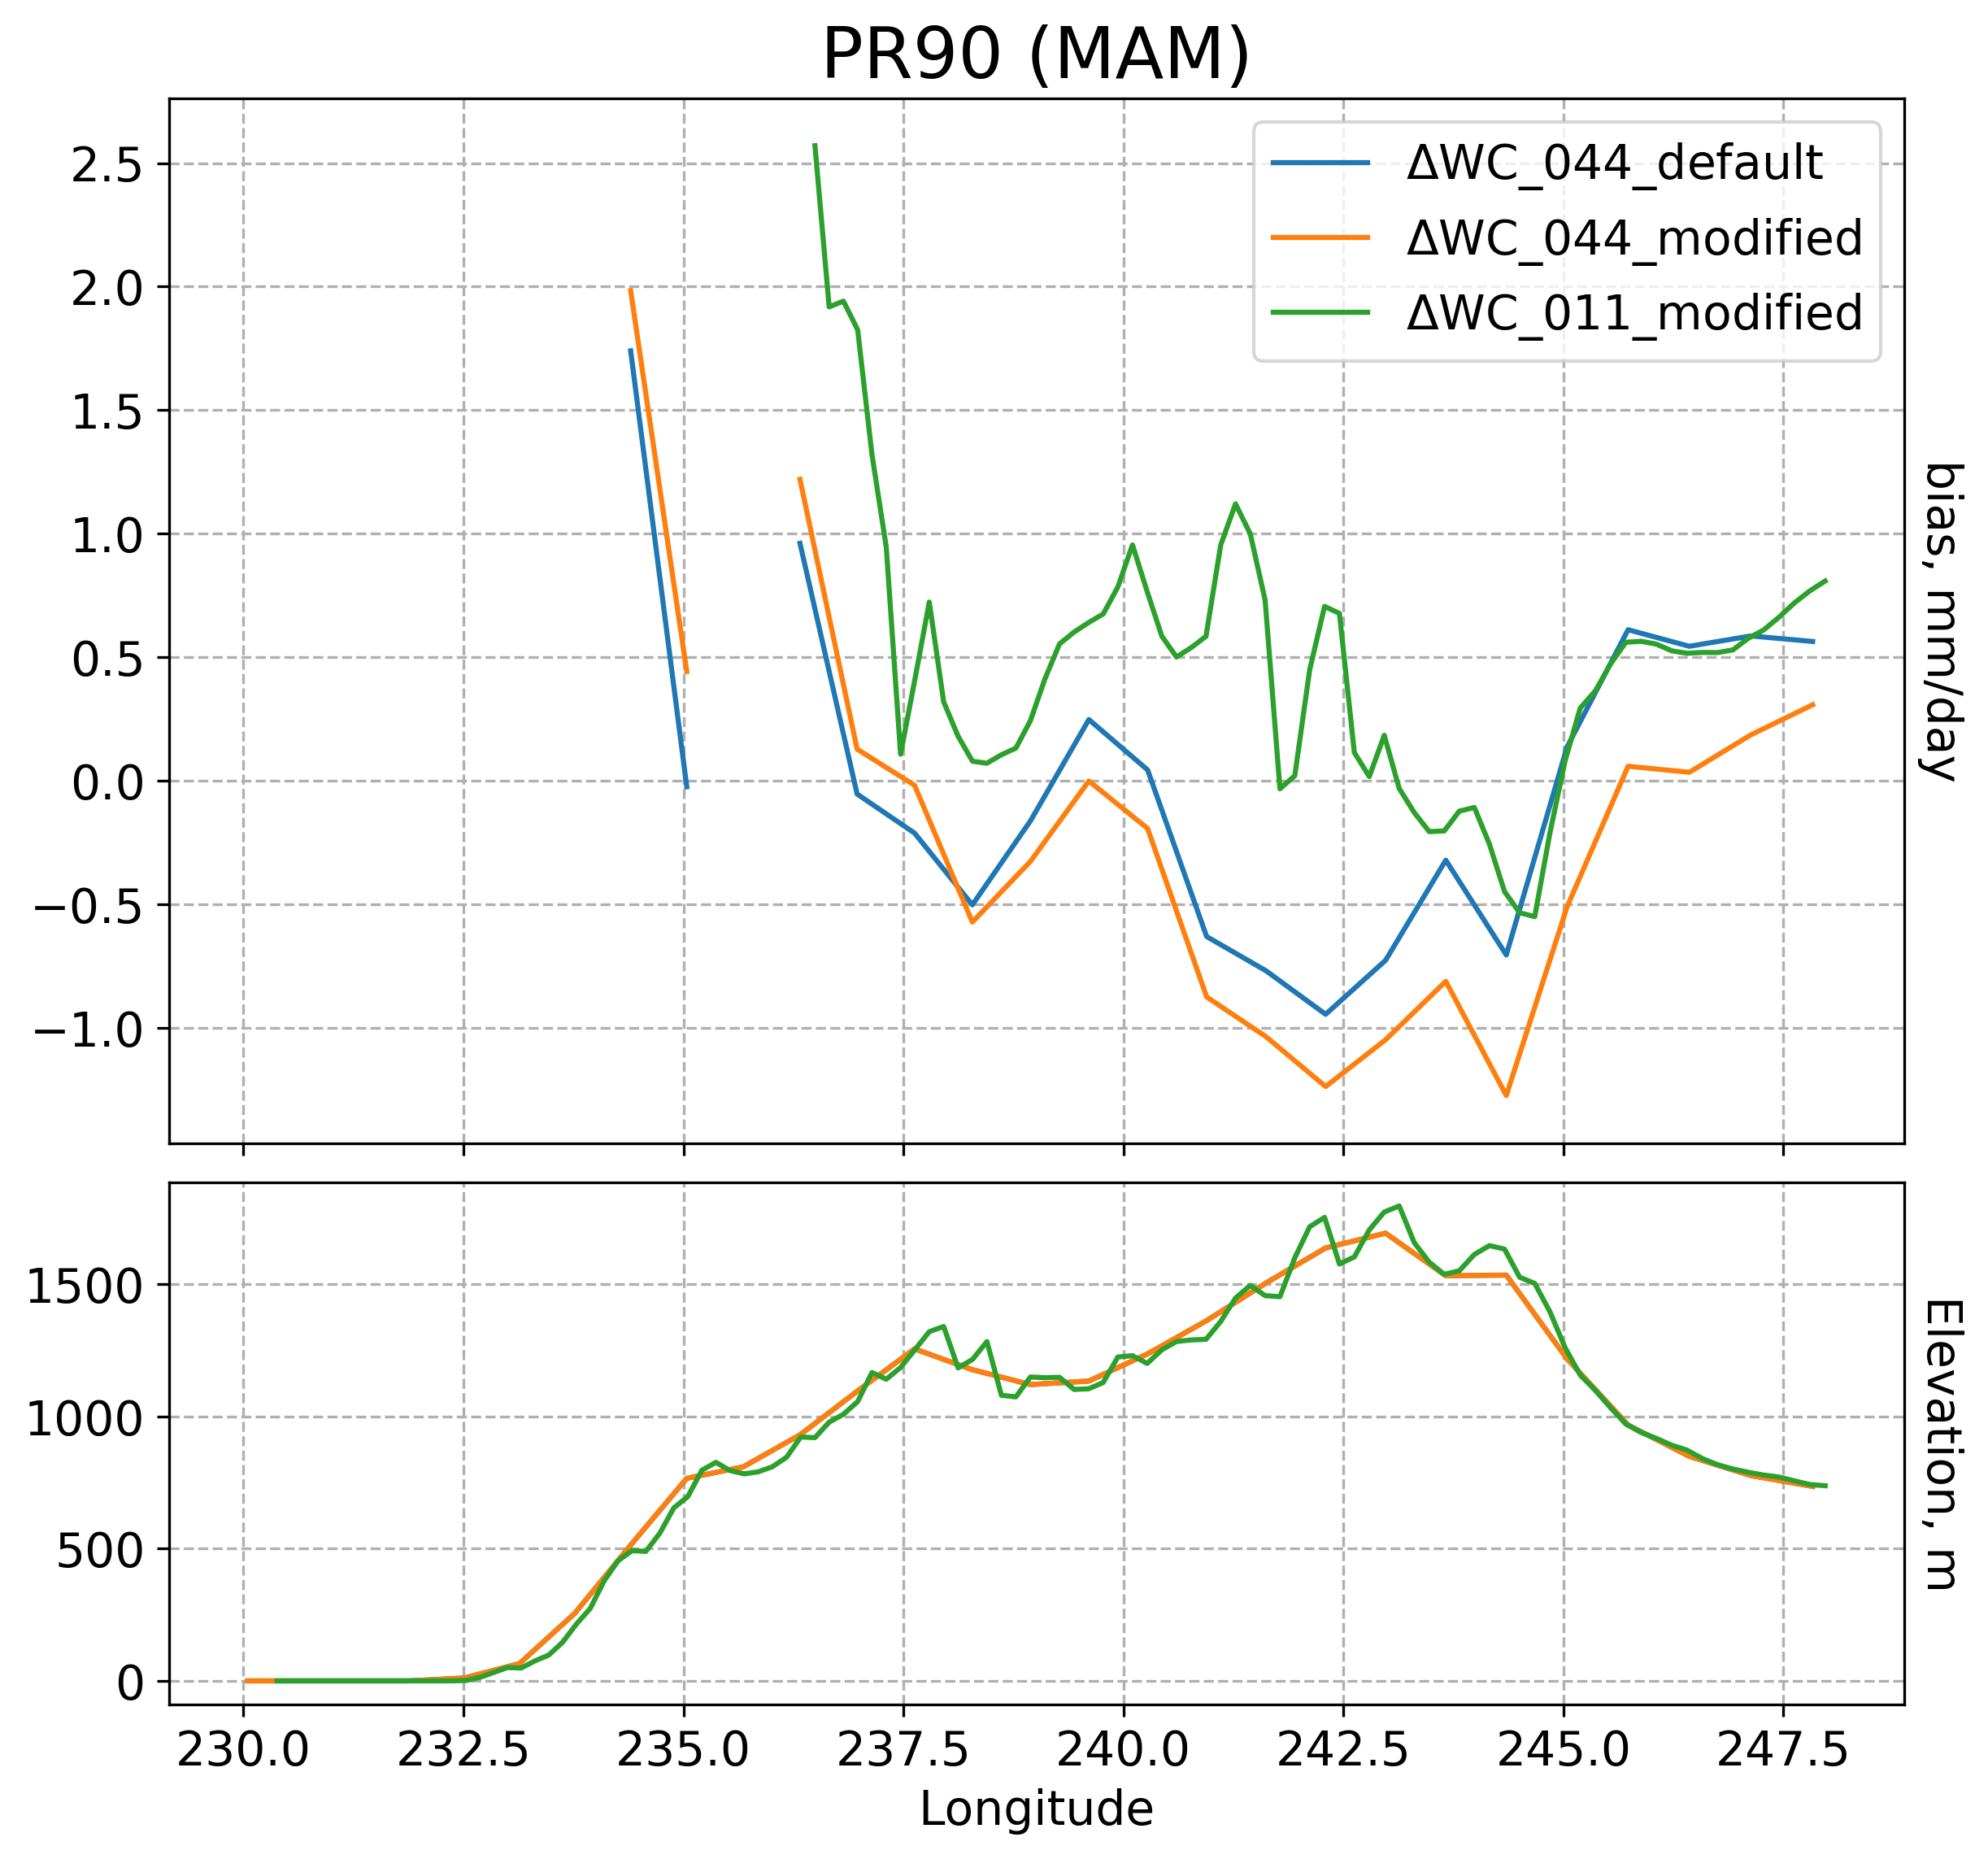
\includegraphics[width=0.31\linewidth, trim={0 0 0 11.5cm}, clip]{figures/meridional_avg/MAM_total_prec}
    % };
    %
    % \node[below=\hspc of tn90_son] (el2) {
    %   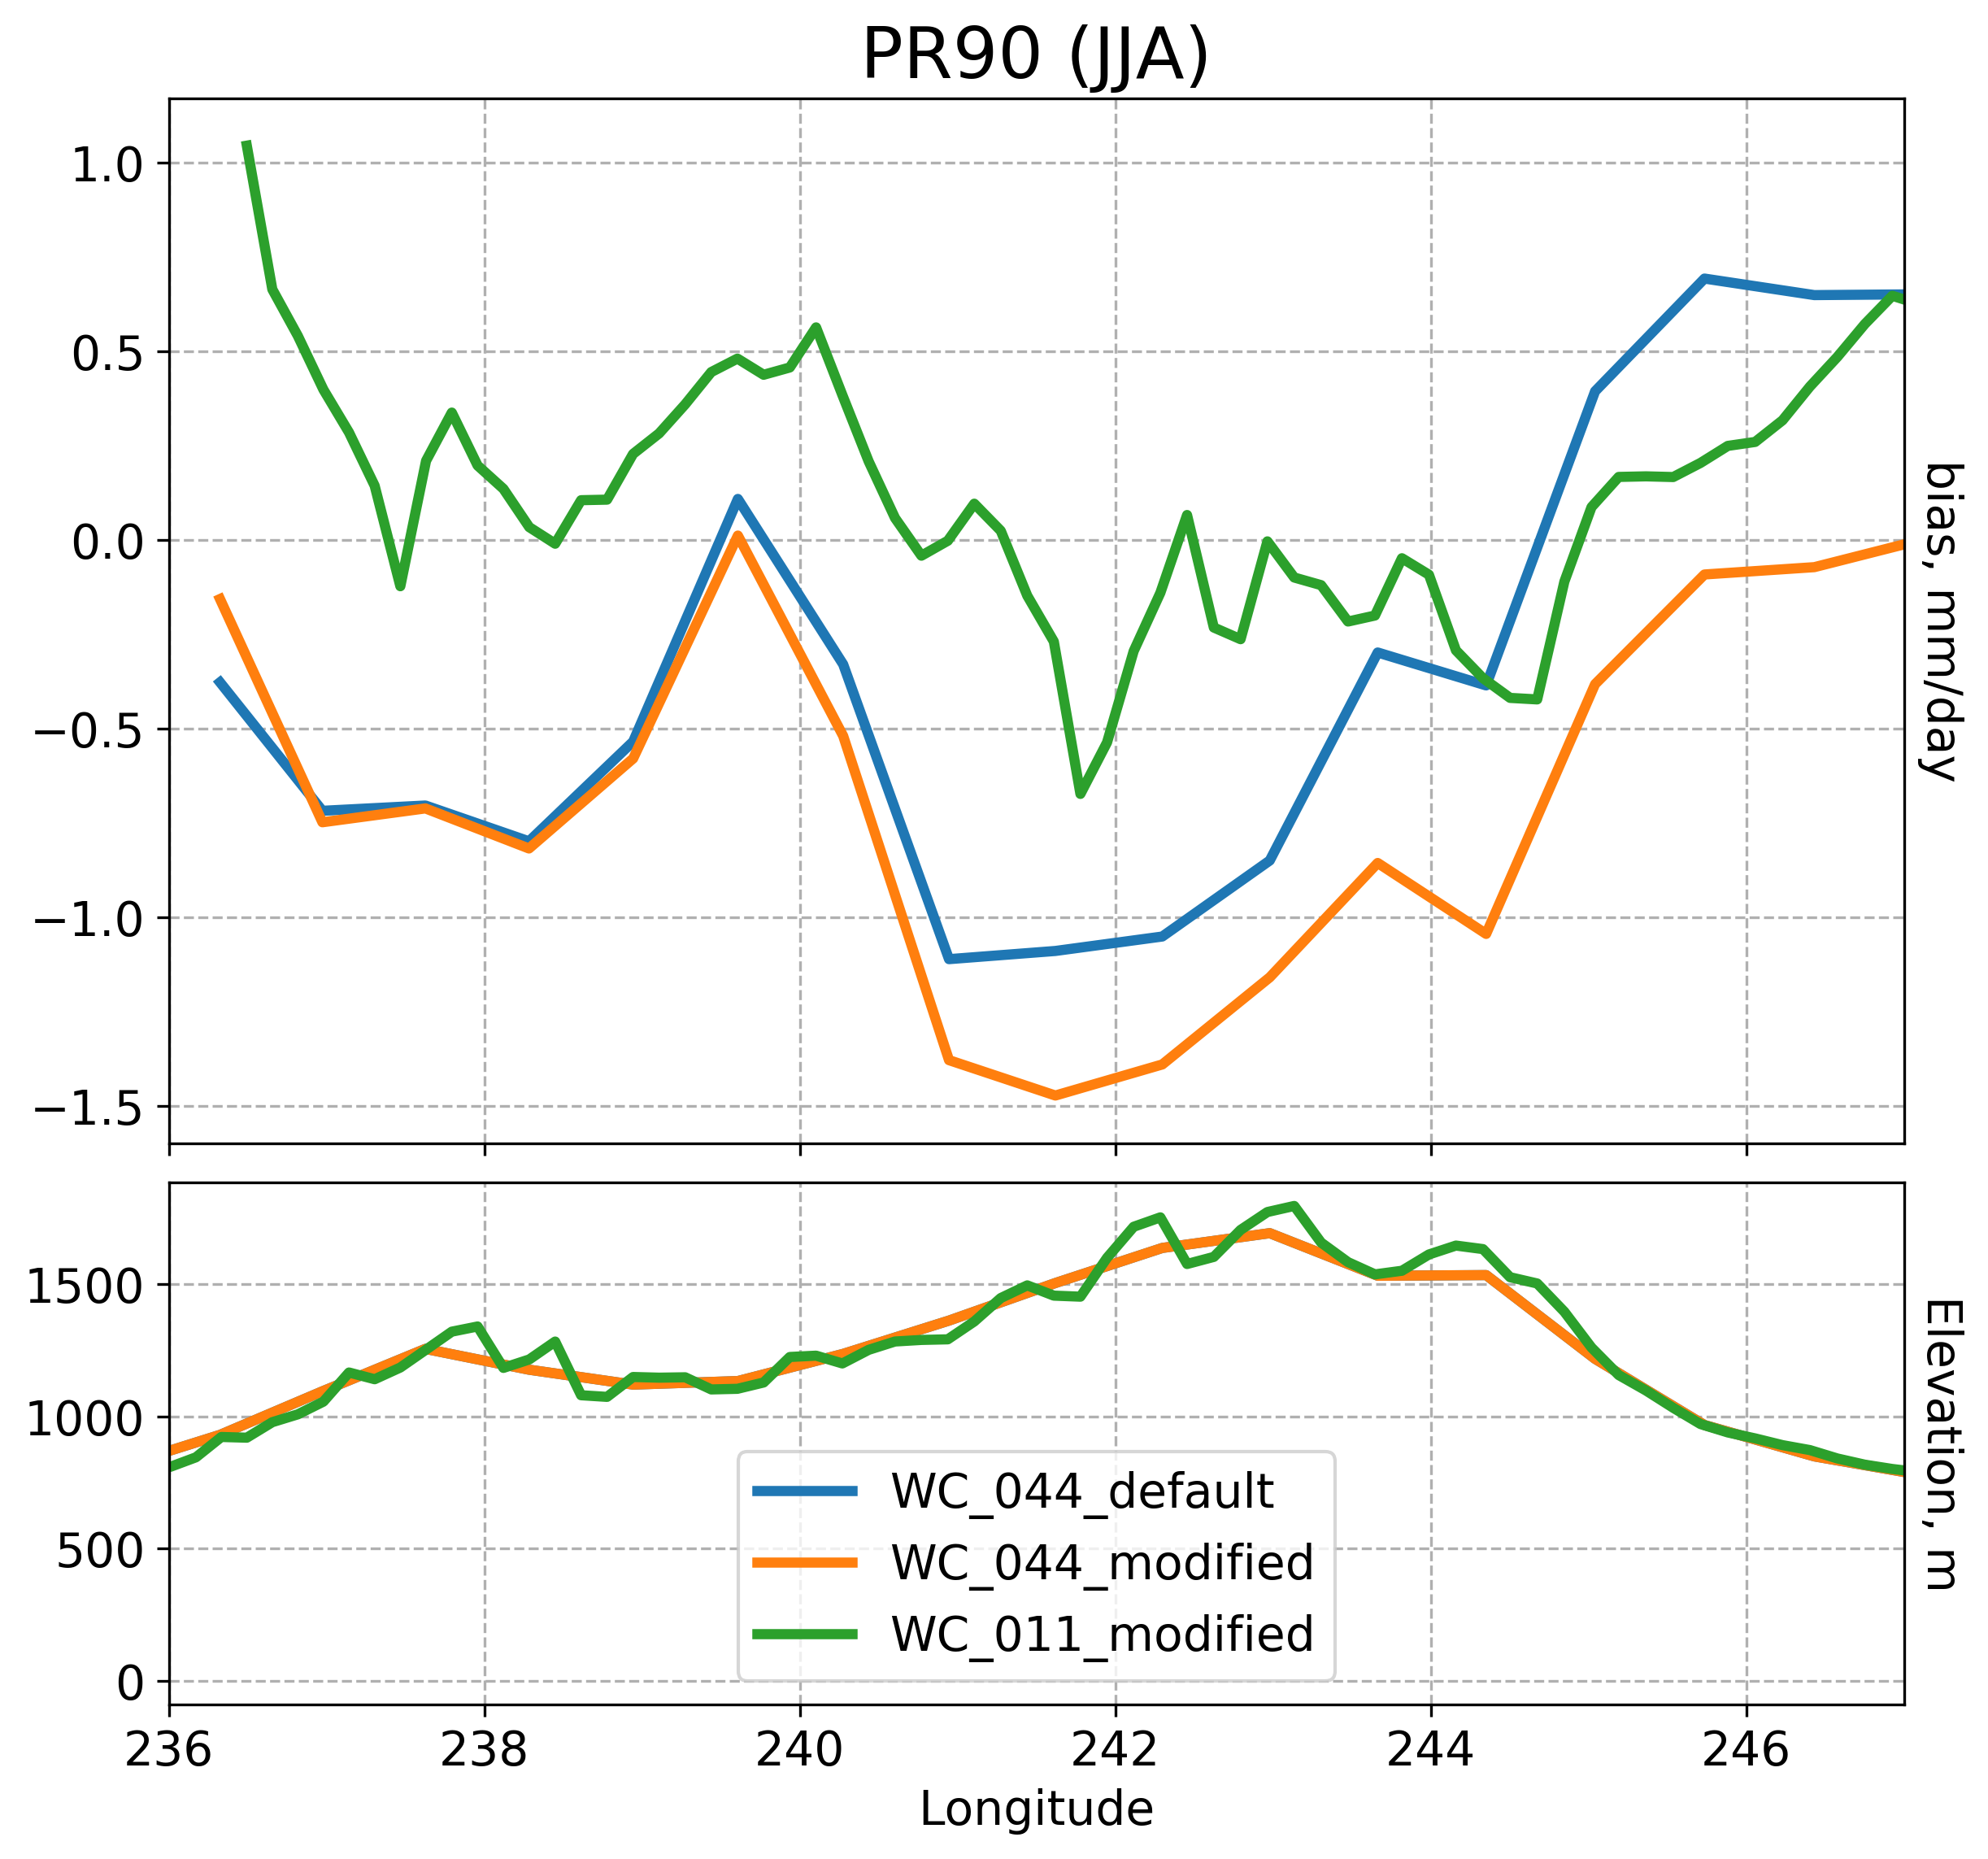
\includegraphics[width=0.31\linewidth, trim={0 0 0 11.5cm}, clip]{figures/meridional_avg/JJA_total_prec}
    % };
    %
    % \node[below=\hspc of pr90_son] (el3) {
    %   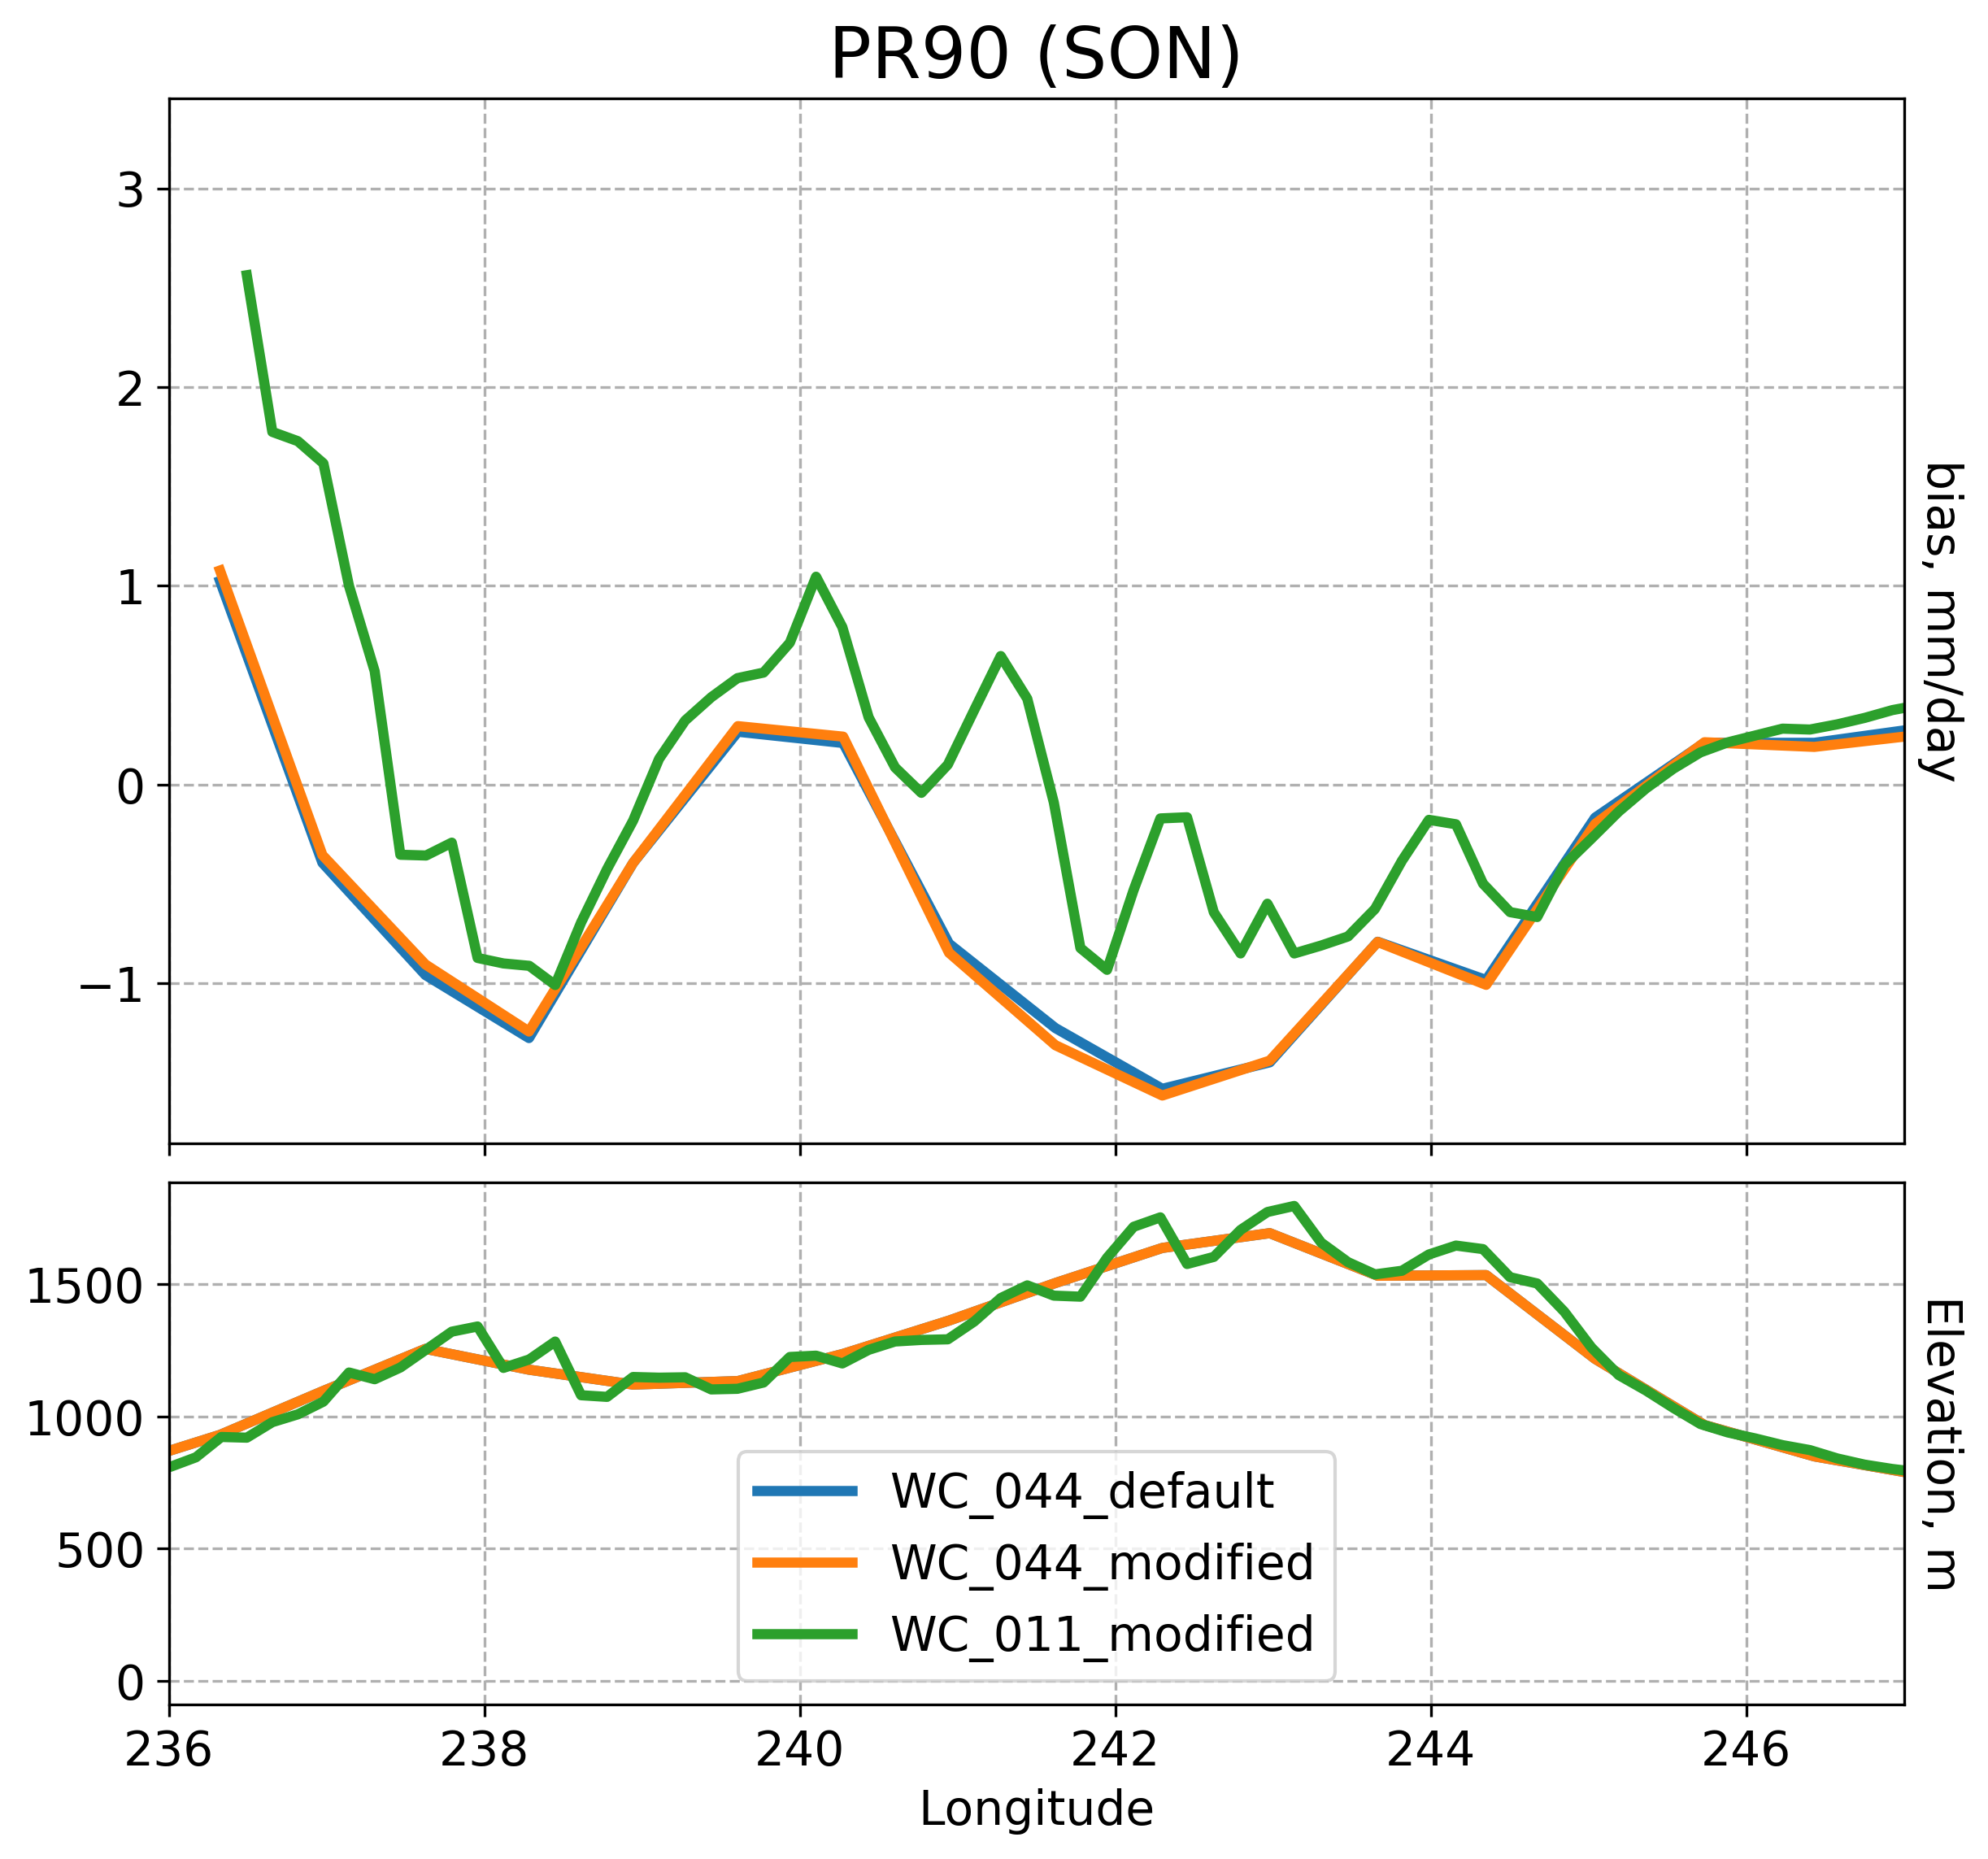
\includegraphics[width=0.31\linewidth, trim={0 0 0 11.5cm}, clip]{figures/meridional_avg/SON_total_prec}
    % };

    \node [below=-0.5cm of tx10_son.south west, anchor=north west, text width=\linewidth, align=left]{
      \captionof{figure}{\color{Green} Zonal structure of seasonal mean biases for 10th percentile of daily maximum temperature (TX10),
      90th percentile of daily minimum temperature (TN90) and 90th percentile of daily mean total precipitation (PR90) for WC\_044\_default (blue),
      WC\_044\_modified (orange) and WC\_011\_modified (green). The biases are calculated using DAYMET observation dataset.
      }
    };


\end{tikzpicture}
\end{center}
\end{minipage}



%----------------------------------------------------------------------------------------
%	CONCLUSIONS
%----------------------------------------------------------------------------------------
{
  \color{SaddleBrown} % SaddleBrown color for the conclusions to make them stand out

  \section*{(D) Conclusions}

  \begin{itemize}
  \item In this project, CRCM5 simulations with newly added surface parameterizations of dynamic vegetation,
  glaciers and frozen soil hydraulic conductivity were evaluated over the region of western Canada at 0.44$^\circ$ and 0.11$^\circ$ resolutions.
  \item It is recognized that the modified configurations are not tuned as extensively as the default one and therefore
  some added value is still expected to be gained after the model is retuned.
  \item Conclusion...
  \end{itemize}
}
%\color{DarkSlateGray} % Set the color back to DarkSlateGray for the rest of the content

%----------------------------------------------------------------------------------------
%	REFERENCES
%----------------------------------------------------------------------------------------
%\nocite{*} % Print all references regardless of whether they were cited in the poster or not
\footnotesize
%\bibliographystyle{plain} % Plain referencing style
\bibliography{sample} % Use the example bibliography file sample.bib
%
%----------------------------------------------------------------------------------------
%	ACKNOWLEDGEMENTS
%----------------------------------------------------------------------------------------
% \section*{Acknowledgements}
% \footnotesize
% This research was carried out within the Canadian Network for Regional Climate and Weather Processes (CNRCWP) project funded by the Natural Sciences and Engineering Research Council (NSERC) of Canada. Computing resources provided by Compute Canada.

%----------------------------------------------------------------------------------------
\end{multicols*}
\end{document}
